% !TEX TS-program = xelatex
% !TEX encoding = UTF-8
\documentclass[12pt, a4paper, titlepage]{book}

\AtBeginDocument{\usepackage{arabluatex}}
\usepackage{tgtermes}
\usepackage{graphicx}
\usepackage{xpatch}
\usepackage[paper = a4paper,
			twoside,
			bindingoffset = 2mm, hmargin = 15mm,
			vmargin = 15mm,
            heightrounded,
			dvipdfm]{geometry}
\usepackage[utf8]{inputenc}
\usepackage[T1]{fontenc}
\usepackage{fontspec}
\usepackage[hidelinks]{hyperref}
\usepackage{amsmath}
\usepackage{rotating}
\usepackage{afterpage}
\usepackage[nottoc]{tocbibind}
\usepackage[backend=biber,
            style=alphabetic,
            ]{biblatex}
\addbibresource{main.bib}

\usepackage{titlesec, blindtext, color}
\definecolor{gray75}{gray}{0.75}
\newcommand{\hsp}{\hspace{20pt}}
\usepackage[myheadings]{fullpage}
\titleformat{\chapter}[hang]{\Huge\bfseries}{\thechapter\hsp\textcolor{gray75}{|}\hsp}{0pt}{\Huge\bfseries}

\setmainfont[Ligatures=TeX,Script=Arabic]{DejaVu Sans}
\let\origdoublepage\cleardoublepage
\newcommand{\clearemptydoublepage}{\clearpage{\pagestyle{empty}\origdoublepage}}
\let\cleardoublepage\clearemptydoublepage

\providecommand{\keywords}[1]
{
  \small	
  \textbf{\textit{Keywords-}} #1
}

\providecommand{\motcles}[1]
{
  \small	
  \textbf{\textit{Mots cl\'es-}} #1
}

\providecommand{\kalimat}[1]
{
  \small	
  \textbf{\textit{\arb{alkalmAt almiftA.hiyaT}-}} #1
}

\usepackage{etoolbox}

% Document
\begin{document}
    \afterpage{\clearpage}
    \setlength{\parskip}{5pt}
    \setlength\itemsep{1em}

    \begin{titlepage}
    \newgeometry{top=0.5in,bottom=0.5in,right=1in,left=1in}
    \thispagestyle{empty}
        \begin{center}
            
\includegraphics[width=100pt]{images/logoEnsa}

            \LARGE{
                \textbf{Graduation Project Thesis}
            }

            \vspace*{0.6cm}

            \normalsize{For acquiring the degree}

            \vspace*{0.4cm}

            \Large
            \textbf{State Engineer}

            \vspace*{0.5cm}

            \large
            \textbf{Computer Science}

            \vspace*{0.6cm}

            \normalsize{Class 2021 - 2022}

            \vspace*{1.2cm}

            \hrule

            \vspace*{0.6cm}

            \Large
            \textbf{Implementation of industrial standards on a SaaS for an MVP for logistics}

            \vspace*{0.6cm}

            \hrule

            \vspace*{-0.5cm}

            \includegraphics[width=125pt]{images/logo}

            \vspace*{-0.5cm}

            \Large
            \textbf{M. Metougui Taha}

            \vspace{0.5 cm}

            \large{presented the 25th of June 2022}

            \vspace{0.5 cm}
        \end{center}
        \raggedright
        \Large
        \textbf{Jury members:}

        \vspace{0.5 cm}

        \normalsize
        M. Medouri Abdellatif \hfill Ensat\'e Professor (President)

        M. Bentajer Ahmed \hfill Ensat\'e Professor (Examiner)

        M. Darraz Othman      \hfill Company Supervisor

        Ms. Besri Zineb       \hfill Ensat\'e Supervisor

        \vspace{1cm}

        \centering
        Academic year: 2021-2022
    \end{titlepage}

    \frontmatter

    \thispagestyle{plain}
    \begin{center}
        \vspace{0.9cm}
        \Huge
        \textbf{Acknowledgements}
    \end{center}
    First and foremost, I am extremely grateful for my parents for their love, prayers and
sacrifices from the time I've been a child to till now, and for their support and
encouragement with my studies and career choices. I am also grateful for my brother 
who has been a source of inspiration and support to me in my life. And my sister
who has always been a great support in my life.

I would like to express my sincere gratitude to my organization supervisor Mr. Darraz
Othman, who guided me in the development of the project and provided me with the necessary support to complete the tasks I was assigned. And especially for giving me the chance of
joining such an ambitious and dynamic project where I learned a lot of new things.

My sincere thanks go to my academic supervisor M. Besri Zineb, who guided me through the
release of this report and put down me on the right path. Also I'm thankful for her
patience, support, encouragement and for all the time she gave us to complete our work
in the right way.

I would also like to thank the CEO of the company I worked for, Mr. Jean-Marie Lespiaucq,
for giving me the opportunity to work with such a great project, and for his encouraging 
and enthusiastic support. And for giving me the chance to play a part in the development
of the project not just as a student but as a professional.


    \afterpage{
        \newgeometry{top=0.2in,bottom=1in,right=1in,left=1in}
        \chapter{Abstract}\label{ch:abstract}
        The logistics has been one of the major industries that's oriented to the
adoption of technology and digitalization for simplifying the work in their overly
complex workflows and helps with their decision making, leading to a overall fast
growth pace. Thus there have been a swarm of new ideas trying to acquire their
share of the market, leading to innovative idea and as we say new sought
solutions, these solutions come mostly as proof of concepts(PoC) or minimum viable products(MVP) as they are cheaper
to produce, and offer a better possbility of creating a product that's more adept to the
needs of the end users. During my graduation project, I undertook the subject of adapting
an MVP to industrial standards, meaning that we transform the MVP into a Software as a
Service(SaaS) which provides multiple advantages for the health of the development of the
product, and the experience of the users.

During the implementation and contribution to the project, I took over the following
tasks.
Persistence of the data specifically archival.
integrating security on the code level as filters to undesired access or spams.
Migrating infrastructure to a containerized environment for better availablity and
scalability.
Implementing deployment strategies within continuous integration and delivery.
Adding new features to the solution that were much needed for the users.

These subjects were the main ones that I undertook during this project, where
we interacted with various tools and technologies, such as Git, AWS toolkit, Docker and
a backend fully focused on Java Spring.

\keywords{
    Minimum Viable Product,
    Software as a Service,
    Fleet management,
    Industrial standards}


        \newpage
        \begingroup
        \let\cleardoublepage\relax
        \chapter{R\'esum\'e}\label{ch:resume}
        La logistique est un domaine o\`u la technologies et la digitalisation ont conduit 
l'innovation dans ce domaine. C'est dû \`a la croissance rapide de cette industrie.
Donc comme c'est un march\'e o\`u l'innovation peu prendre \c{c}a place et que les 
nouveau projets ont pu prendre leur part. C'est pour cette raison o\`u des solutions
MVP sont cr\'ees pour bien comprendre les besoins des utilisateurs et bien s'adapter
au domaine au fur et \`a mesure de la cr\'eation de ces solutions. Donc durant mon 
projet PFE j'ai int\'egr\'e le sujet de l'indistrualisation d'un MVP, c'est \`a dire
d'adapter un MVP aux normes des SaaS. C'est \`a dire transformer le MVP en un SaaS qui
offre plusieurs avantages pour le cycle de vie de la cr\'eation et d\'eveloppement de
la solution, et l'exp\'erience des utilisateurs.

Durant la r\'ealisation de mon projet PFE, j'ai pris le r\'ole de suivre les diff\'erentes
t\^aches, allant d'impl\'ementation des bases de donn\'ees pour la conservation des
donn\'ee et l'archivage. Int\'egration des normes de s\'ecurit\'e au niveau des filtres
de l'application. Et puis, nous avons migr\'e l'infrastructure d'une  machine virtuelle
linux vers des images Docker d\'eployer sur des contenaires AWS. Et Finalement, nous
avons ajout\'e des fonctionnalit\'es pour la gestion des utilisateurs.

\motcles{
    Gestion de flotte, MVP, SaaS, Standard industriel}

        \endgroup
        
        \newpage
        \begingroup
        \let\cleardoublepage\relax
        \setRL
        \chapter{\arb{mulaxa.s}}\label{ch:molakhas}
        \setLR
        \begin{arab}
    'in majAl alUjistIk mina almajAlAT alra'iIsIT almuwajahT 'ilA alta.hawul
    altiknUlUjI. muwa-jihaTaN 'i`timAdaha `l_A raqomanaTi m`.zami `amaliyAtihA
    bihadafi tab.sI.tihim, 'aw 'isti`mAl ha_dihi al'axiraT fy 'an.zimT tusA`ido
    fy `itixA_di alqarArAt. wa bi_dalika laqad 'adat 'il_A watyraT numuw jid
    sarI`aT, wa limo.sAyaraT ha_dA alta.Tawur alsarI` wajaba `al_A al^sarikAt
    alnA^si'aT w almubtakirIn al'i`tmAd `al_A .turuq tumakinuhum min ta.hqiq
    .hulUlihim w 'afkArihim bidUn al'iltizAm alkAml bi bina2 albinyaT alkAmilaT
    (PVM), wa ha_dA yumakinuhum min ma`rifaT al'i.htyAjAt bi^sakliN
    tadrIjI. li_dA xilAla ma^sru`i taxarjI, qumtu b'itixA_di mawodU` takyIf
    barnAmajo (PVM) 'il_A alma`AyIr almunAsibaT. h_dihi alma`AyIr torakizo
    `l_A qAbiliyaT altaws`, al'amn wa binyaT t.htiyaT .sulbaT.

    xilAl `amaly, laqad ta.taraqt 'il_A mawA.dI` muxtalifaT, minhA
    'i`dAd qawA`id albayAnAt xA.saT bialar^sIf. wa.d` qawA`d al'amn
    `an .tarIq wa.d` .toroq li'iqAf hajamAt (SODD), wal.had mn 'imkAnyT
    aldxUl 'ilA lil mostaxdamIn. tm_A ta.taraqnA 'il_A ja`l albiniyT
    alta.htyaT 'iftirA_dyT tatamakano min tawzi` almawarid
    wa 'idArT alni.dAm bi^sakliN tilqA'iY.
\end{arab}
\setRL
    \kalimat {
        MVP, SaaS, \arb{'idArT al^s.hinAt}
    }


        \endgroup
    }

    \afterpage{
        \newgeometry{top=0.75in,bottom=1in,right=1in,left=1in}
        \chapter{Acronyms}\label{ch:acronyms}
        \begin{table}[!htpb]
    \centering
    \begin{tabular}{| c | c |}
        \hline
        API & Application Programming Interface\\
        \hline
        AWS & Amazon Web Services\\
        \hline
        App & Application\\
        \hline
        CD  & Continuous Delivery\\
        \hline
        CEO & Chief Executive Officer\\
        \hline
        CI  & Continuous Integration\\
        \hline
        CLI & Command Line Interface\\
        \hline
        CTO & Chief Technology Officer\\
        \hline
        DB   & Database\\
        \hline
        DDOS & Distributed Denial of Service\\
        \hline
        ECR  & Elastic Container Registry\\
        \hline
        ECS  & Elastic Container Service\\
        \hline
        HTTP & Hypertext Transfer Protocol\\
        \hline
        IP   & Internet Protocol address\\
        \hline
        IT   & Information Technology\\
        \hline
        JS   & JavaScript\\
        \hline
        JVM  & Java Virtual Machine\\
        \hline
        JWT  & JSON Web Token\\
        \hline
        KPI  & Key performance indicator\\
        \hline
        MQTT & Message Queuing Telemetry Transport Protocol\\
        \hline
        MVP  & Minimum viable product\\
        \hline
        OAuth & Open Authentication Protocol\\
        \hline
        OOP  & Object Oriented Programming\\
        \hline
        PoC  & Proof of concept\\
        \hline
        RATP & Régie autonome des transports parisiens\\
        \hline
        RDS  & Relational Database Service\\
        \hline
        REST & Representational State Transfer\\
        \hline
        S3   & Simple Storage Service\\
        \hline
        SCM  & Supply Chain Management\\
        \hline
        SCP & Secure Copy\\
        \hline
        SOA  & Service Oriented Architecture\\
        \hline
        SSH & Secure Shell\\
        \hline
        SSM  & Secrets Management\\
        \hline
        SaaS & Software as a service\\
        \hline
        VPS  & Virtual Private Server\\
        \hline
    \end{tabular}
\end{table}

        \begingroup
        \let\cleardoublepage\relax
        \listoffigures

        \listoftables
        \endgroup

        \tableofcontents
        \clearpage
        \restoregeometry
    }
    
    \mainmatter

    \chapter{General Introduction}\label{sec:introduction}
    Minimum Viable Products (MVP) has seen a rapid rise in popularity, and it is
now one of the most popular to take on new projects that present a risk.
MVP is a set of guidelines for creating a product which focuses on validating
a product idea with customers early in the development lifecycle, it normally
contains enough features and functionalities to be usable and setup a ground
for the development of a product for later stages. And relies on early adopters
to help the product reach its full potential. However, opting for such an approach,
can be turn into a heavy load on the development team, if development keeps on expanding
on the product without opting to set a strong foundation to be strongly maintainable.

One way to tackle that is to opt for adapting the MVP to industrial standards,
turning it into a SaaS product. The industrial standards are a set of norms that
are set by the industry to have a strong foundation for the development of a
product, to be able to be easily maintained and allow to turn the MVP into more of
an actually rigid solution. For example, taking one of the most popular and famous
companies in the world, Amazon, the industry standard for software development. The main
idea of the project was selling books online and that started with a minimalistic operated
online store rather than a full fledged e-commerce store. Just to make sure that
the idea is properly tested on the market, then it have been industrialized to match
a fully built online books store with a strong foundation, which later turned out to
be a full on e-commerce not store but rather a infrastructure.

In the course of my graduation project, I present report is a brief overview of adapting
parts of the MVP foundation to industrial norms. On the basis of this, we will be able to
see how the MVP can be adapted to the industry standards, and how it can be used to create
a SaaS product that can be more secure, more reliable and easily maintained.

Through the course of this report, we will be introducing the context of the project,
the problem that's we're facing and the solutions that we're going to propose and implement
to solve them.



    \chapter{Context and Problematic}\label{sec:context}
    The reliance on automated and self-sustaining systems is increasing especially
in the fields of logistics, finance, and manufacturing. But there are still many
manual processes that need to be addressed for management aspect. This is where
automation steps in where every repeatable human process can be dropped into an
automated workflow.

The company I'll be partaking in this internship is "ONAR MMSoft" which is a company
specialized in developing workflow management services for three core activities,
which are catering, logisitics and industry. For my subject, we'll be focusing mainly
on the logistics aspect, where they already offer a Minimum Viable Product (MVP)
for the management of fleets flow within factories.

So during this internship, I undertook the subject of industrializing a Minimum
Viable Product (MVP) for a logistics company, which presents the challenge of
turning a usable Proof of Concept (PoC) into a rigid, reliable and scalable Software
as a Service (SaaS), and to handle this process in a structured way, we'll be following
the kanban method.
\newpage


    \section{Introduction}\label{sec:context_intro}
    At the growth rate multiple industries are going through, it's no secret that the reliance
on automated and self-sustaining systems is increasing especially in the fields of
logistics, finance, and manufacturing. Targeting more specifically the supply chain
logistics, the industry is looking for solutions that can automate decision making
processes of moving goods from one place to another, ones targetting efficiency increase
for warehousing and distribution networks, others diving into security aspects of the
supply chain, or even managing the flow of goods and services including a bunch of
processes for transformation of raw materials into marketable products within logistics
which is what we call \emph{SCM} or Supply Chain Management.

But even with all this automation in hand, there is still many time consuming and manual
processes that need to be addressed precisely for management aspect.

So here where automation steps in, every repeatable human process can be dropped into an
automated workflow that can be executed in a timely manner or triggered as a on demand
service. Providing a unified interface for all the processes, the automation can be used
to automate the entire supply chain.

Thus came in my decision to partake in the development of a product aimed for the
automation of the fleet management process within factories with "ONAR MMSoft".



    \section{Host organism}\label{sec:host-organization}
    The company ONAR MMSoft is a company that located at Jouy-en-Josas, France.
It's part of a bigger company, ONAR MMCall, which specializes in the distribution of pagersm, in as a complement to this offering software that can blend with the pagers.

As of today, the company has worked in several fields of activities:

\begin{center}
    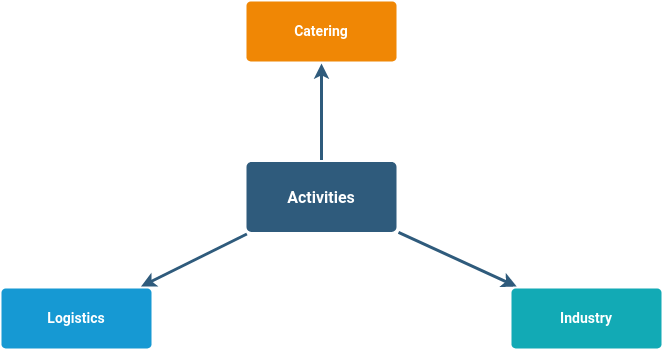
\includegraphics[width=0.8\textwidth]{images/core_activities.png}
\end{center}

Mainly handling the problems of management of part of the workflows in all these fields. 
And lately turning all their focus to logistics as their field of interest.

\begin{center}
    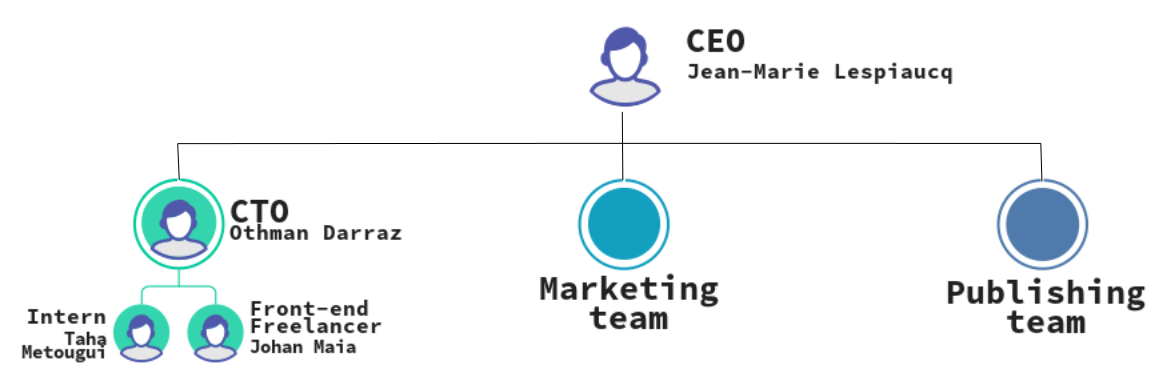
\includegraphics[width=0.85\textwidth]{images/Hierarchy}
\end{center}

The team, I've integrated, is composed of a team of 2 people, the CTO Othman Darraz who's in charge of managing the project
and a freelancer Johan who's in charge of everything that's front related, and me joining them as the third
member of the team taking care of backend mainly refactoring, optimization and security.




    \section{Problematic}\label{sec:problematic}
    As said before in section \ref{sec:context_intro}, there's a clear lookout for automation
and easing management of the flows within logistics and the organisation came with
a solution to this problem, but as it's just an MVP, it's still missing some points
in terms of security, flexibility and rigidness.

To start off, an \emph{MVP} is a minimum viable product, which is a product that
is designed to be used in a limited number of situations and it's first aim
is providing an actual product to the customer and then use it to know learn
the behavior of the users and gain some understanding their interest \cite{MVP_def}.

\begin{figure}[h]
    \centering
    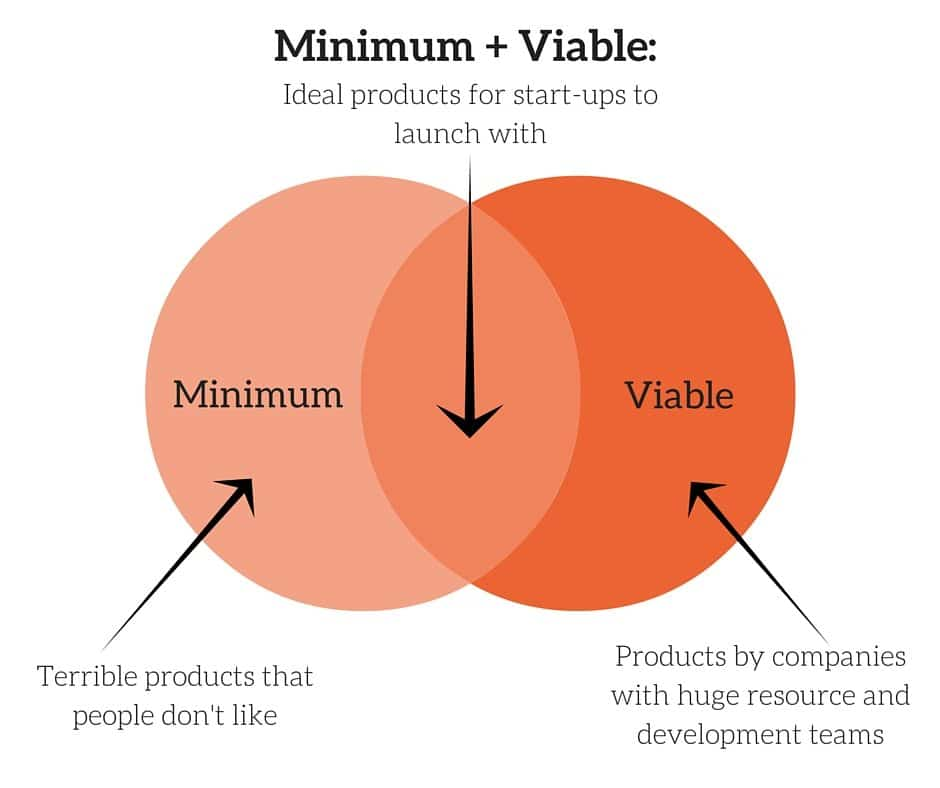
\includegraphics[width=0.6\textwidth]{images/Minimum-Viable.jpg}
    \caption{\footnotesize{Concept of a Minimum Viable Product - \cite{MVP_def}}}
    \label{fig:mvp}
\end{figure}

So going from this definition, it can be clear that a full fledged rigid
solution is never the aim of an MVP, but rather it's just a starting point
for a progressive and flexible solution and for the organization it came in
perfect as this application came in as a subject of a competition and
also the team is small so they didn't have the resources to finance
the creation of a big project. But going for the premise of building as you go,
but this came with it's own drawbacks, leading to a product stuck in the development
hell for too long as there are no clear guidelines for quality and security, so it's
not good once it takes too long and start becoming a costy solution to the creator
with no way to compete in the market.

So here comes the need to implement industrial standards and guidelines, which
is the aim for now, these standards are as follow:
\begin{itemize}
    \item \emph{Security}: Implement a security layer to protect the data
        and servers from unwanted visitors and attacks.
    \item \emph{Flexibility}: Creating a flexible solution, that's easy
        to use and extend by the client for their desired functions rather
        than having to develop and adapt the software each time.
    \item \emph{Maintainable}: Make the solution as easy to maintain,
        update and to pickup bugs.
    \item \emph{Automated deployment}: Make the solution deployable in an
        automated way, encouraging testability of the solution before it's
        deployed to any environment.
    \item \emph{Rigid solution}: Creating a solution as rigid as possible,
        so that it can tend to heavy load, have close to no down time and
        be more stable during peak times.
\end{itemize}

By implementing these standards, the solution can easily turn from an MVP to
a robust SaaS, which can be used in production and can be competitive in
the market.




    \section{Work methodology}\label{sec:work-methodology}
    To tend to this challenge, the team has decided to work with the
Kanban method, Kanban is a workflow management method that helps organization
manage and improve work systems, it originated in Japan. Firstly used by Toyota
as a scheduling system for just-in-time manufacturing, it was later adopted by
many other organizations to take toll on software industry in the 21st century, 
it's a flexible and agile method that can be used in many different situations,
for more information \cite{kanban_def}.


The tasks were divided into the following categories:
\begin{itemize}
    \item Stand-By: For non-urgent tasks, or that are not ready to be worked on.
    \item Requested: For tasks that are ready to be handled.
    \item In Progress: For tasks that are being worked on.
    \item To Review: For features or tasks that were done,
        and should be either reviewed or tested.
    \item Done: For tasks that have been completed.
\end{itemize}

\begin{figure}[!htpb]
    \centering
    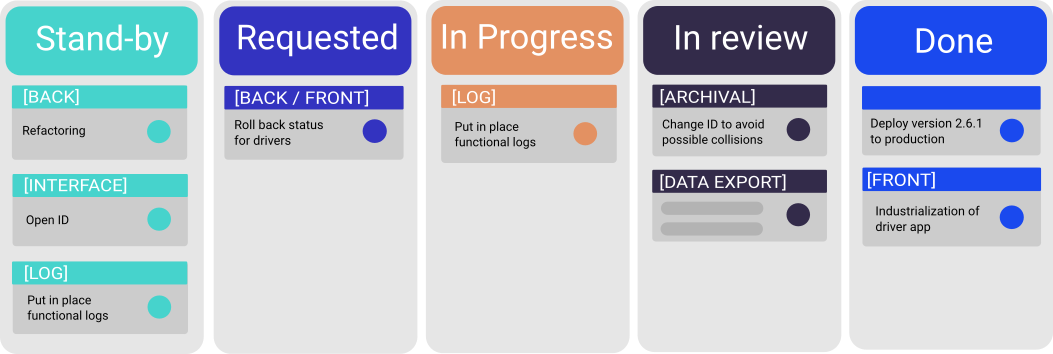
\includegraphics[width=\textwidth]{images/kanban_mod.png}
    \caption{Kanban board elements}
    \label{fig:kanban-board-elements}
\end{figure}

The board was handled using Jira, which is a web-based project management tool developed
by Atlassian that is used to track and manage the development of software projects,
allowing for a wide range of flexibility within the application.

Choosing the features to be implemented in the system was a challenge,
as there were specifications to be followed, and the requirements were
kind of wild and not realistic for the given time frame.

So prior to beginning on the kanban board, there were a few meetings 
mainly to discuss features within the specifications which were to be implemented 
in the system and which were to be kept on hold.

The creation of the tasks then was handled either by the product owner or the project
manager, and giving each one a priority, and a due date was assigned once the task was
picked up and studied for the implementation to assess the proper manner to handle it.

For the reviewing of the tasks, it was decided to be moved to done once the task was
tested thoroughly by the product owner trying to find any issues that may have
passed through the testing done by the developers.

\begin{figure}[!ht]
    \centering
    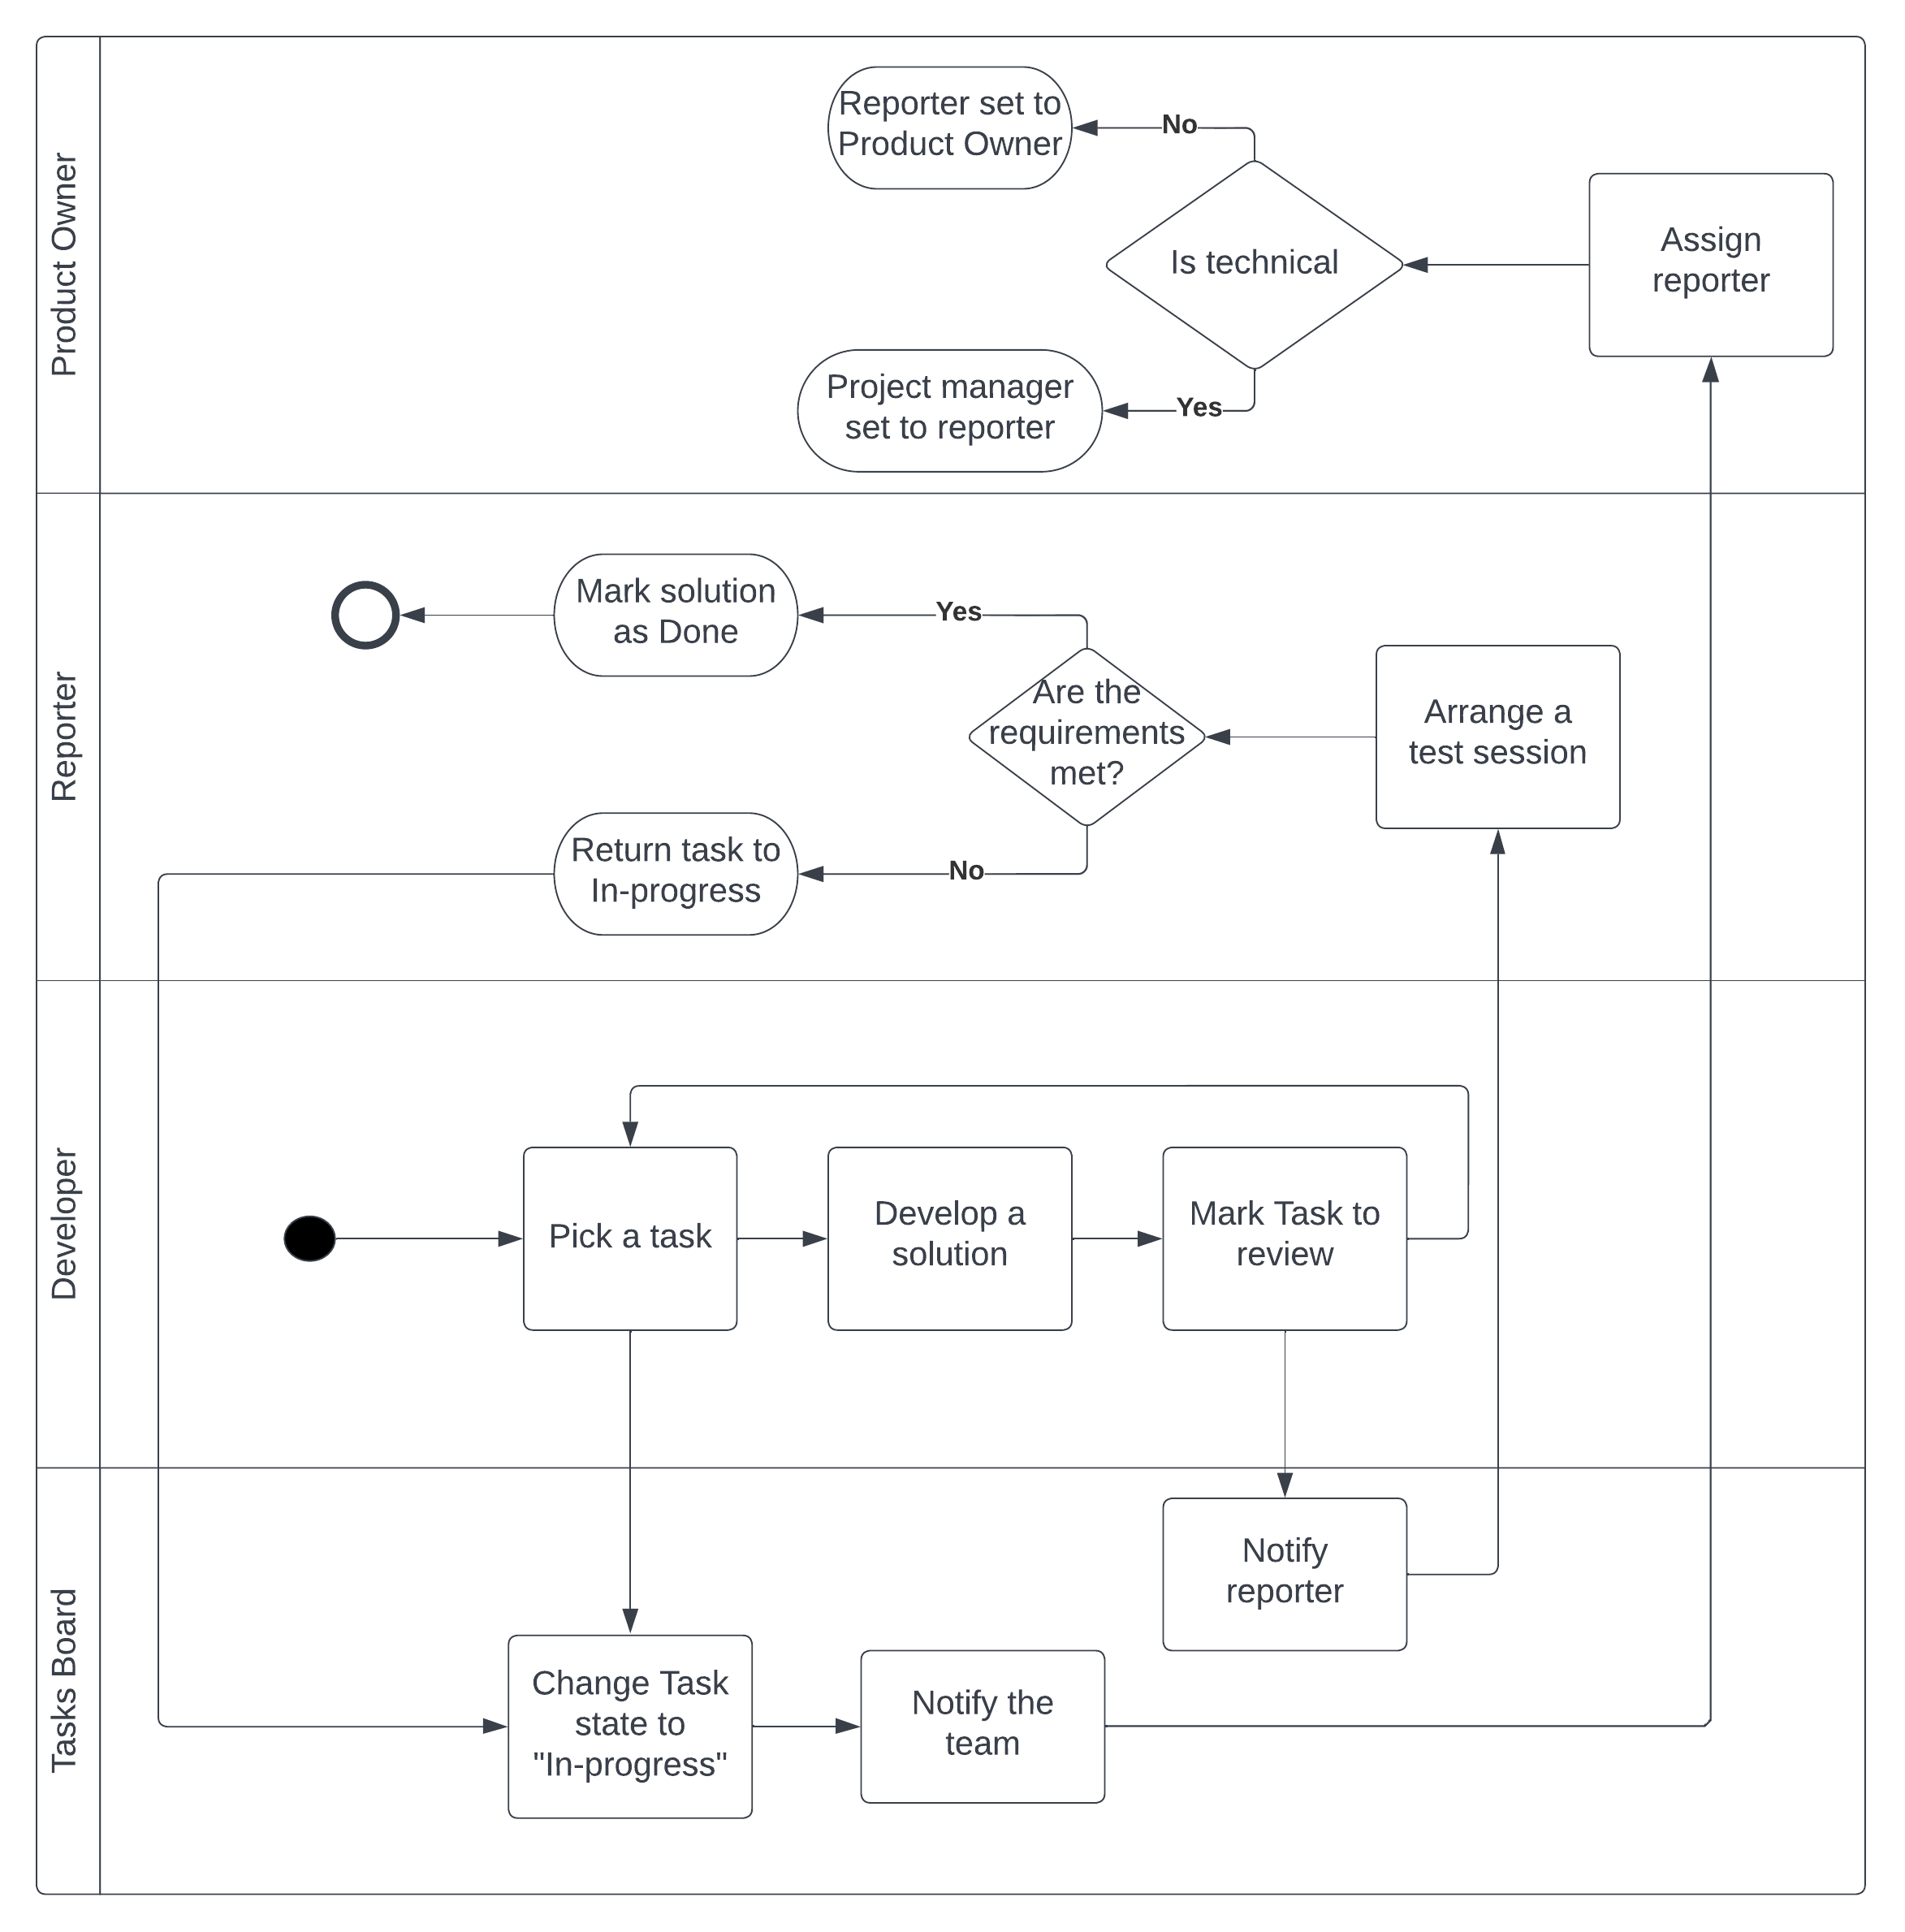
\includegraphics[width=\textwidth]{images/task handling flow.png}
    \caption{Task handling - flow chart}
    \label{fig:task_handling}
\end{figure}

During the development the tasks handling went as showing in figure \ref{fig:task_handling}
and the order was as follows:
    \begin{itemize}
        \item Pick up the task from the requested list.
        \item Task get assigned to the developer who picked it.
        \item Task is moved to the in progress list.
        \item Once done the task is moved to the to review list.
        \item Once reviewed the task is moved to the done list.
    \end{itemize}

For the reviewing of the tasks, it went in two ways, one for the product owner to
review the task when it's related to some business logic or frontend interactive task
and the other for the CTO to review the ones relating to the backend logic and purely,
technical tasks.

\begin{sidewaysfigure}
    \centering
    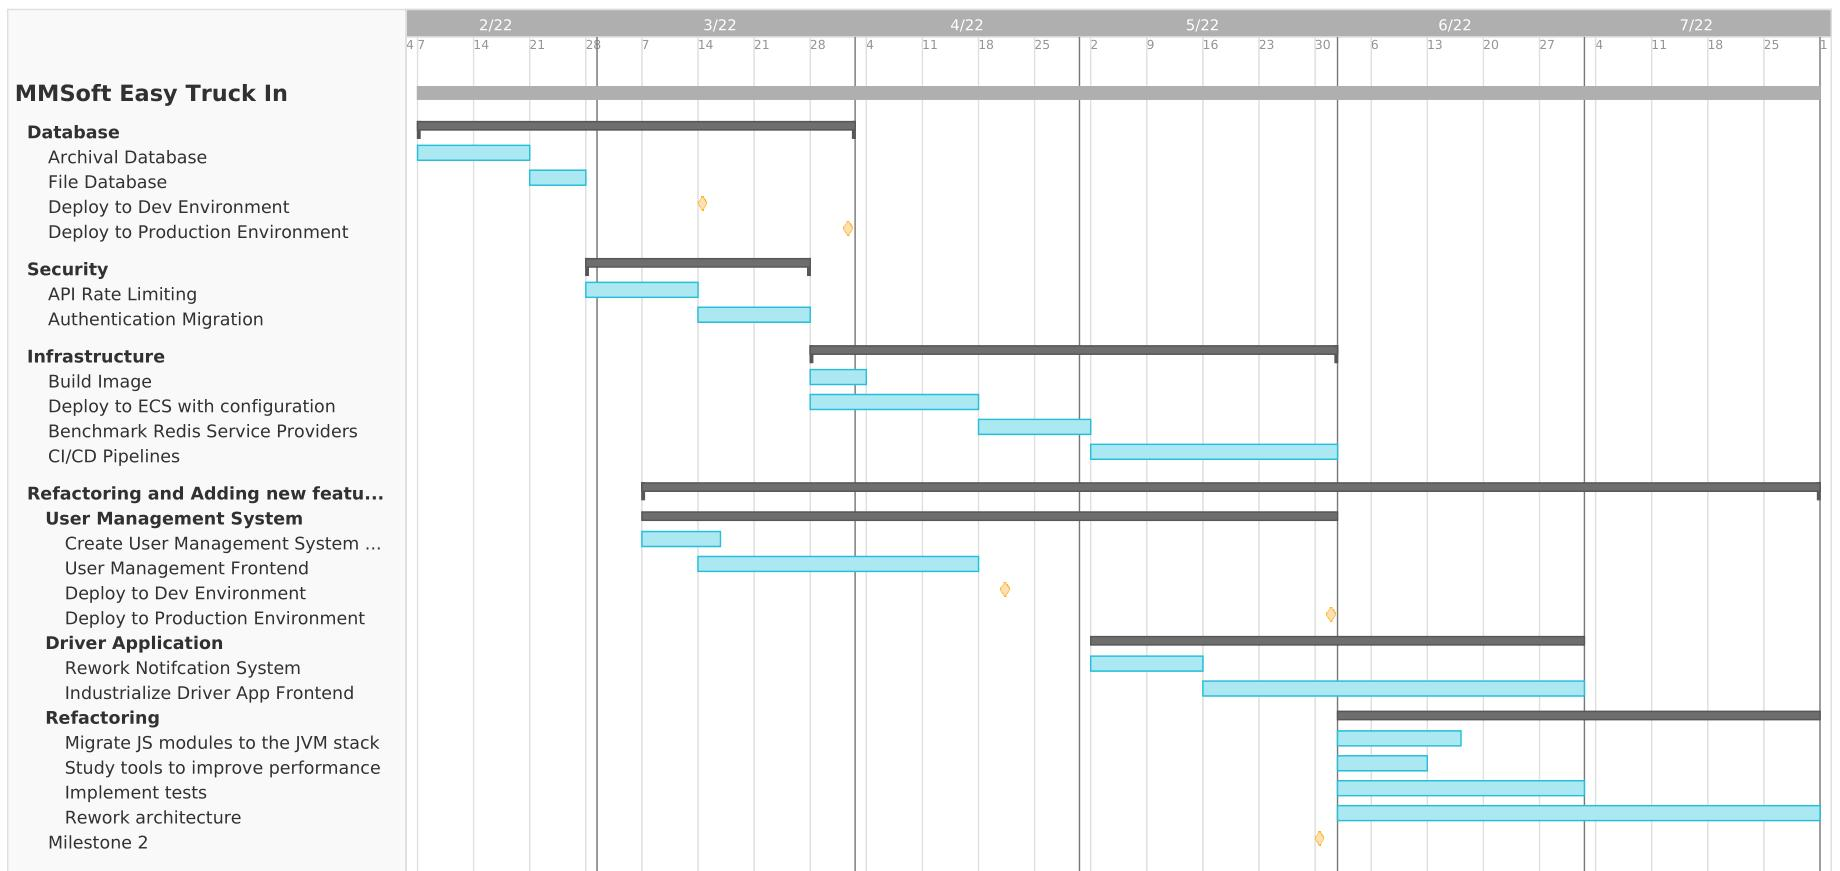
\includegraphics[width=\textwidth]{images/Plan.jpeg}
    \caption{Gantt chart of the project}
    \label{fig:gantt_chart}
\end{sidewaysfigure}

For the forecast plan, it had multiple tasks and milestones planned out as shown in the
\newline figure \ref{fig:gantt_chart} there is the following:

\begin{itemize}
    \item Databases: The solution required specific new features related to data
        to implement. The first one being archival of clients data,
        and the second is the ability to store files and both these
        came with a cost for storage in mind.
    \item Security: Which had multiple layers of security to be handled,
        one of them was handling the authentication of the users to make it
        less exploitable, the other managing the access to the system and
        last rate limiting the api gateway.
    \item Infrastructure: The solution required a new infrastructure, specifically
        one that would allow for the deployment of the system in streamlined
        manor, and also the ability to scale the system through peak times.
    \item New Features: The solution required new features to be implemented,
        which were not a nice to have but rather a necessity, and these were
        addition of a User management system and notification system.
    \item Refactoring and testing: as discussed before the solution came as an
        MVP which required refactoring and testing to be done.
        This part came with a lot of work in mind, firstly a studying of the
        existing tools and libraries to be used, and compare them to the already
        used ones, also the code base was missing a lot of tests for the exisitng
        features so it needed a to have every part of the code have it's own
        tests implemented to ensure the consistency of the behaviour.
        And finally, a rethought architecture of the code base to make it 
        more future-proof and maintainable.
\end{itemize}

\section{Conclusion}

To sum up we've discussed so far the scope of the project, which is taking place
within the "ONAR MMSoft" company, specifically within their product Easy Truck In (ETI)
which is a software application that is used to manage the trucks in warehouses.
The problem with this product is that it's still just a PoC at the moment and they 
are planning to expand their product to a wider audience, which would necessitate 
making it more robust and scalable product, specifically one that would be following
industrial SaaS standards and standards for the software industry.


    \chapter{Assessment of the current state}\label{sec:current_state}
    In this following chapter, we'll be looking at the current state of the whole system.
Taking a look at the current business process, which is constituted of the following
core activities:
\begin{itemize}
    \item Driver handling from accessing the warehouse to leaving it
    \item Digitalization of documents
    \item Secure access to logistics platform
    \item Dashboard for the management with the following functionalities:
        \begin{itemize}
            \item Truck status
            \item Driver status
            \item Document status
            \item Notification system
            \item Guidance system
        \end{itemize}
\end{itemize}

Also we'll be taking a look at the core services provided by the system which are
currently made of four front-end services a web-interface, a mobile application and
a IOT oriented front. Four back-end services a MQTT broker for communication, orchestration
service for real-time data management, registration service for the drivers and trucks,
and a API exposer for integration and last two databases one for handling data storage and the other for handling realtime-data.

Currently the main technologies used are React, Angular and Cermate for front-end,
and Spring, NodeJS for backend modules and all of this is hosted within the hosted
services of AWS.
\newpage

\section{Introduction}

As the solution is already an existing one, we'll be diving into the current state of
the system. Taking a look at the business process, then moving to the core services
explaining the goal of each of them. Then we'll be looking at the current state of the
backend architecture with some overview around the databases and technologies used, and 
why they are used.

Then on the second part of the chapter we'll be taking into account the already existing
system, to build a better understanding of it choices and have some constructive criticism
to take a look at parts that could be improved.


    \section{Analysis of the solution}\label{sec:assessment-of-current-state}
    \subsection{Assessment of current Business process}\label{sec:business-process}
    So for the business process, as stated previously, we have a set of activities that organizes the trucks and their drivers.
In the goal of have them work rather optimally in an automated fashion.

And it goes as follows:

\begin{center}
    \includegraphics[width=0.8\textwidth]{images/flowchart}
\end{center}

As seen in the diagram, it is rather a simple flowchart, but that would require to have a lot real time data put in place,
to have it coordinate with the trucks and drivers, without any downtimes.
And to adapt to the needs in hand, they've put in place the following IT infrastructure:

\begin{center}
    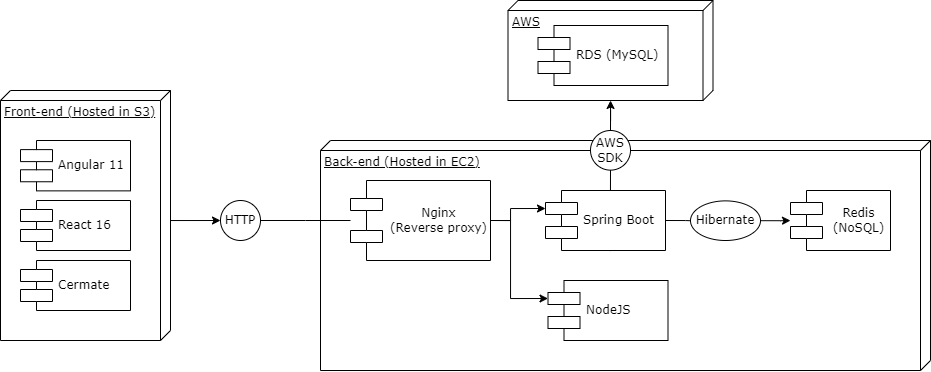
\includegraphics[width=0.8\textwidth]{images/State-of-art}
\end{center}

There are a lot of things that can be done to improve the performance of the system, but the main thing is to have a
base for the proof of concept.
As such, the released IT infrastructure is a good starting point for the proof of concept.

    \subsection{Provided services}\label{sec:analysis}
    Having to take care of managing multiple trucks, truck drivers, their turns, their parking lots
and their parking spaces can be a difficult task to achieve, especially when you have to deal with
time management, availability, delays, and so on.
However, going by old systems, either an Excel spreadsheet or just a ledger system on
paper, can help such a task, as long as you're working on a small scale. But once
this scales, the need for assistance grows.

And that's the point where comes the possibility to make use of automated tasks to do the job.
Automating the management, making it easier to manage with as little human intervention
as possible.

As of the current time, there is already a solution put in place, which is a SaaS hosted
on AWS implementing an SOA architecture. The SaaS relies on various managed services
provided by AWS, such as EC2, S3, RDS, etc.

The MMSoft Saas is constituted of:
\begin{itemize}
    \item Four front-end services:
    \begin{itemize}
        \item Easy-truck-in (ETI) interface which is the main interface
        \item Driver application (Angular 11)
        \item Registration Tablet App (React 16)
        \item Gatekeeper App (Cermate)
    \end{itemize}
    \item Four Back-end services:
    \begin{itemize}
        \item MQTT Broker communicating with the Gatekeeper app (VerneMQ)
        \item Orchestration Back-end Service (Java 11 Spring Boot 2.6) used by the ETI interface
        \item Registration Service (Node JS 16) used by the Registration Tablet App
        \item TMS Registration Back-end which exposes REST API for integration (Java 11 Spring Boot 2.6)
    \end{itemize}
    \item Two databases:
    \begin{itemize}
        \item MySQL for users, site, configuration
        \item Redis as a database for Daily/Weekly data and for messaging communication with other services
    \end{itemize}
\end{itemize}


And it has the following backend service used, as shown in the figure below:

\begin{center}
    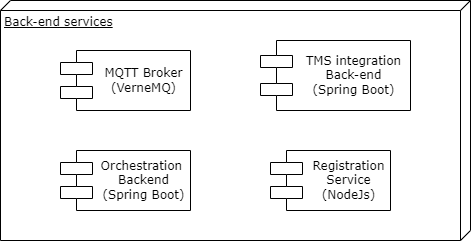
\includegraphics[width=0.8\textwidth]{images/Backend}
\end{center}





    \subsection{Conceptual model}\label{sec:conceptual-model}
    As of now the software is still in it very early stage, and being used mainly as a proof of concept.
And it's following the architecture below:

% TODO: this needs to get reworked
\begin{figure}[!htbp]
    \centering
    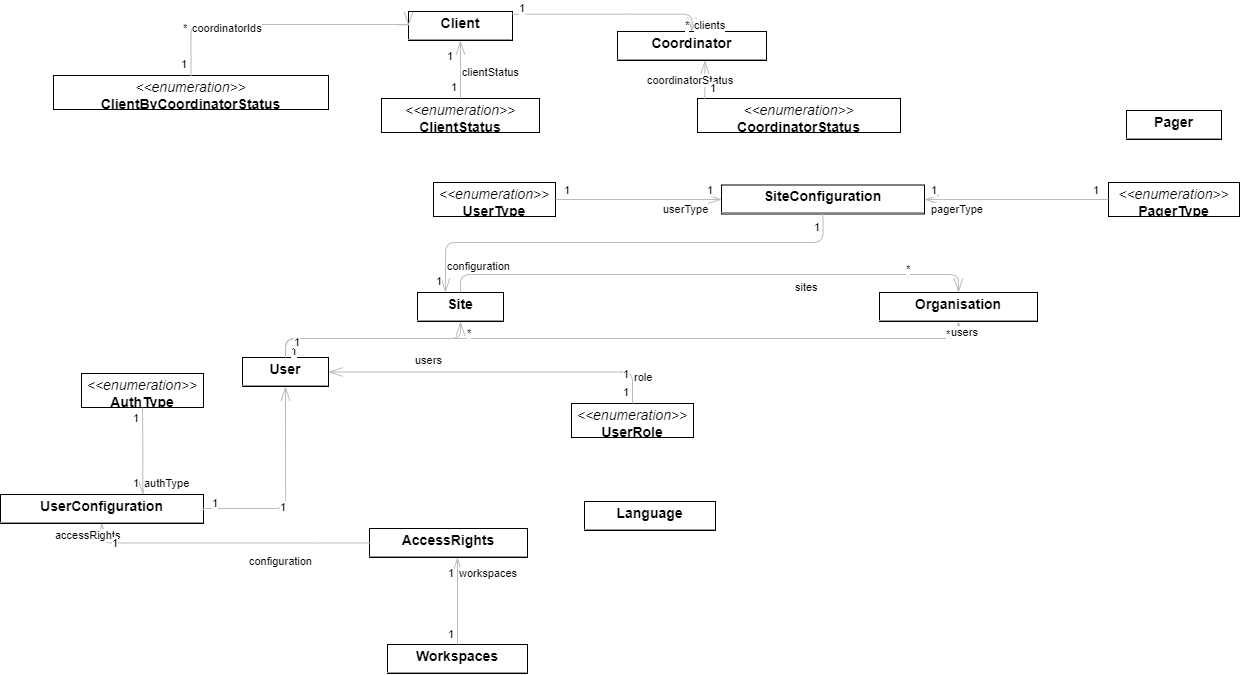
\includegraphics[width=1\textwidth]{images/package.drawio}
    \caption{\footnotesize{Backend model}}
    \label{fig:backend}
\end{figure}

% TODO: This part will be updated once we take on the subject of refactoring.



    \section{Criticism}\label{sec:criticism}
    With the general structure of the software present, it is clear that the
software is missing some important features and building blocks that can make it 
the SaaS it's aimed to be.

To start with the essentials, as the software is targeted to be used for logistics
within factories and warehouses, it's important for the data of daily interactions and
operations to be stored in a database and be accessible to analytics and KPI's operations
to be able to provide a better understanding of their efficiency and how their
work is flowing. Because for the mean time, all the daily operations data is being stored
in the Redis database and Redis being an in-memory data structure store used as a database,
message broker, and streaming engine \cite{redis_def} it won't be suited for long term storage
as to keep it operational it will need to clear old data and free up space, thus why it's cleared
on a daily to weekly basis. And with no archival solution put in place, the data for now is
cleared then lost which means for any client opting to pull their old data for analytics
won't be possible.

Next comes the user management system, which is clearly a key factor in such a workflow, 
as seen in the \ref{fig:flowchart} there are multiple actors involved in the process,
from the gate keepers, operators, drivers, and the management staff. So with the current
user system which opts to have user set as a site which means for each factory there's a
single user or even though you can make multiple users they all will have full permission
in the site's scope which isn't secure neither is a good idea. So opting to a new system
which encourages the use of a role system for users and the users then belonging to a site
would be a better solution, as it would even open the flexibiltiy of adding configuration
to the user roles, and have each user have their own scope of permissions depending on
their role.

Also for the authentication, the current system uses a Bearer token which is a Json Web
Token (JWT) and that is permanent rather than an ephemeral one. So if an attacker manages
to intercept a token, which in fact is doable with code injections to expose a request,
then they can use it to access the backend at any time.
Opting to some other authentication system, such as a cookie based system, would be more
secure, as the cookies could at least be held in a secure place such as code injections,
can be used to acquire them from the front-end.

Looking at the current system and how the deployment is done, which is done in a manual way,
so it's takes more time to deploy simple bug fixes and new features reducing from the efficiency
of the developers, due to the time it takes to deploy each time. For fact, it's clear that
the addition of some automized deployment tools would be a good way reduce the need for the
manual deployment and also allow for faster deployment of new features and hot-fixes as the
deployment process is mostly a recurrent set of actions.

Next comes the code quality, which is rather messy, as it uses a lot of different tools,
some part are just redundant which could be done in a DRY\footnote{DRY or don't repeat
yourself is a term used to describe the practice of writing code that is not repetitive.
It is a way to reduce the amount of code that needs to be written.\cite{pragmatic_bro}} way,
not to the extreme of course where the code is becoming DRY but in expense of readability
and complexity. Other than the redundancy of some parts, the use of different approaches
in the code can get kind of messy and hard to maintain, especially if you're not familiar
with the code which would be the case in the expansion of the team, so the more the code
is unified the better. Also the code is not documented, so it's not clear what some parts
of the code internals do when it's something complex and that requires a modification.
The tests for the majority of the code are not put in place, so in the case of huge update
to the code, it would not be possible if some behaviour changed or if some parts are just 
not working.

There's the usage of different tech stacks which are NodeJS and Java Spring, which is a bit
of a mess, as it's not clear why the NodeJS is being used in the backend without much impact
as it's just handling some simple backend logic that could migrated to a Java Virtual
Machine(JVM)\footnote{JVM is the virtual machine that's capable of running Java binary
code}, compatible language such as Java, Kotlin, Scala, \dots, why I said a JVM compatible
language it's because the majority of the system is built on Java so it would make it
easier to migrate Js to Java than let's say moving the Java to NodeJS, but also to gain
the advantages of strongly typed language making it easier to pick up bugs. With such a
move, it would create a more uniform and rigid way to have the whole project fully handled
with single build tool, which in turn can really ease up the deployment process, and make
it automatable more easily.

One other point to tackle is security within the code, the current code base uses secrets
which are stored directly in the code, which is not secure, as you can easily acquire the
original code through a decompiling tool, or even through a reverse engineering tools,
which would make those secrets attainable directly. Opting for some other way of storing
the secrets, such as a database in addition with environment variables, would probably be
a better solution, in addition with a rolling system of secrets in possible cases making
those keys temporary.

\section{Conclusion}

To summarize the current state of the software, it's clear that the current application
is at in terms of the features and the current state of the code, it's clear that there's
a strong foundation for the application to be a SaaS as it's already handling almost the
full workflow of the fleet management system, , but there are some missing features and
building blocks specifically in the infrastructure and security aspects, which could be
mediated to complete the organization view of their product.


    \chapter{Our contributions}\label{sec:implementation}
    For the contributions, we had multiple subjects and points within the solution touched on,
which as follow:
\begin{itemize}
    \item Persistence Layer: Which took interest in the implementation of an archival 
        system for the solution, it went in two different ways:
        \begin{itemize}
            \item Implementing the archival for general data that was in JSON format.
            \item Implementing the archival for data that was binary files such as PDFs.
        \end{itemize}
    \item Security Layer: It was the part where we implemented a new filter to the backend,
        specifically for limiting the call backs to the API, through a rate limiter.
        And next was the authentication, which was a migration from a simple Bearer token
        transactional method to a more secure method based on Http Only Cookies storage for
        the token.
    \item Infrastructure: This part mainly targetted, migrating the environment from linux
        virtual machines to managed containers that could offer a better scalability,
        in terms of managing peak load for requests and memory usage.
    \item Continuous integration: Here we implemented a CI/CD pipeline for the solution,
        which took advantage of the previously implemented containerized environment.
        To make the deployment more streamlined and efficient, to allow for easier hot
        fixes and upgrades, and force a better testing of the solution before allowing 
        code to be deployed in an automated fashion.
    \item Refactoring: This was the last point, where the main goal here is to make
        the code more readable and easier to maintain. The trade off is that it will
        take a long time to implement as it requires implementation of a lot of tests
        for the old code. To allow for the beginning of the re-implementation of the
        code, to a newer version that relies on a different architecture.
\end{itemize}

\newpage

\section{Introduction}

So with the context, the problematic and the scope of the project setup, it's 
time to pass to the contributions phase, which consists of conceptual contributions
and their implementation. To be more precise, we'll be handling persistence layer,
security layer, the infrastructure layer and a new deployment strategy.

For each of these layers and phases, we'll be starting with a conceptual or theoretic
study of the solutions we have, and then we'll be talking about the implementation 
projecting it to the project to finally move to the testing and how it was done to validate
the solution used.

\section{Target}\label{sec:target-comp}
As of the current moment the forecast component diagram for the system is as follows:

\begin{center}
    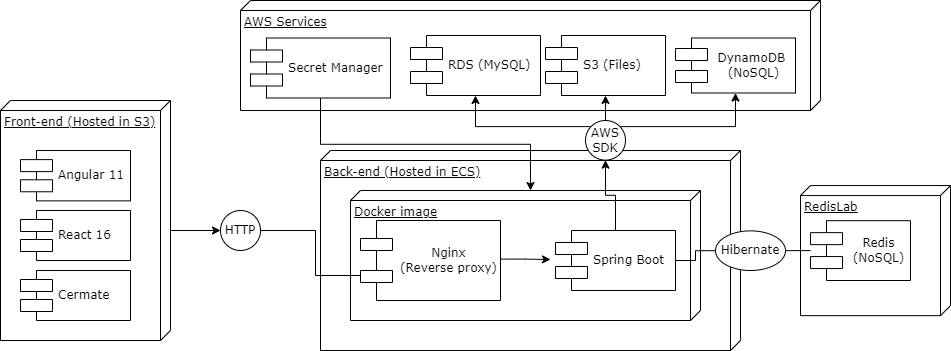
\includegraphics[width=0.8\textwidth]{images/forecast}
\end{center}

As it shows there are additional databases mainly ones for archiving files as is the case of
S3 and also archiving data for statistics down the line thus using DynamoDB\@.
Also containerizing the backend for the goal of having it run different instances seamlessly,
and have the run times duplicate efficiently.
For the creation of the images, it should be noted that they will be generated automatically,
and upload to ECR directly through CircleCI pipelines.
Thus the process of having to update or fix bugs within the back-end will be more streamlined
in a fashion that causes little to no downtime.


\section {Persistence layer}

For the database we had two subjects to study:
\begin{itemize}
        \item Databases for archival purposes
        \item Databases for storing files
    \end{itemize}

\subsection {Archival Database}
So taking the first one, we had to study performance to cost of three solutions and their scalability:

    \begin{itemize}
        \item RDS (SQL)
        \item DynamoDB (NoSQL)
        \item Aurora (SQL)
    \end{itemize}

As all three were AWS solutions, the performance of each was pretty much the same,
and as the database was going to be used for archival it relied less on having a
high throughput and more on how much storage costs.
So we only relied on the cost of the solution, how easy is it to maintain.

So going off by cost first Aurora was the most expensive, with no value added to the problem we'll be solving with it.

So that left us with two options:

    \begin{itemize}
        \item RDS (SQL)
        \item DynamoDB (NoSQL)
    \end{itemize}

We dived into the RDS solution, and it was a bit of a challenge to get it to scale,
in terms of storage compared to DynamoDB which offered autoscaling options and variable
throughput for high load time which could fit the needs of archival as it could take 
higher input in the daily backup process, than the rest of the day.
And for the output there wasn't much to be gained, for neither of the solutions as it was
a rare process that wouldn't be used alot only on demand by the user.

Going to studying the cost, the primary tool that was used for that is the AWS Cost Calculator, which gives rather good indicators to approximate the charges.

\textbf{Case study: }

For the data we used the following:
- 200 Entries per site.
- 500 Site.
- 2 KB per entry.

Site represents the factories and the entries represents the trucks.

So with those inital values, we came to the following results:
- Daily storage of 200 MB or monthly of 6 GB that increments after the period passes.
- 3000000 writes / month
- 100000 reads / month

the reads were just second guessed as there was no significant data about it, 
other than it will be a low read database.

So for the calculations, for RDS we used the following options:
- Instance db.t3.large (vCPU: 2 Memory: 8 GB)
- Instance reserver for one year 
- Single-AZ (1 node)
- 6 GB storage incremented monthly
- 6 GB backup incremented monthly

which resulted in the yearly cost of \$1185.769

For DynamoDB, we used the following options:
- Standard-Infrequent Access (Reduces cost of storage)
- 3 Mil writes per month
- 100K reads per month
- 6 GB storage incremented monthly
- 6 GB backup incremented monthly

Which came down to the cost of \$236.00 per year.

As we can notice the RDS cost was much higher than DynamoDB,
so we decided to use DynamoDB as it was cheaper, and also had
better maintenance options offered by AWS as it's a fully hosted
service.

Lastly, the only missing part was integration within the back-end which went on different steps.

First we had to create a service on the Spring Back-end that took on the handling of the communication layer between the DB and the back taking on mulitple functionalities such as:

    \begin{itemize}
        \item Creating - delete tables
        \item Creating indexes to allow fast access to the data
        \item Adding - deletting data
        \item Finding data using specific fields
    \end{itemize}

Then implementation of unit tests for the service to ensure that it's working as intended,
it had taken on the following tests:

    \begin{itemize}
        \item Create table for tests with required indexes
        \item Adding data to table, and then finding it
        \item Adding data to table, and find it by date
        \item Adding data to table, and find it by different keys
        \item Cleaning up the table
    \end{itemize}

The creation of the tables and their indexes was automated, to allow for the
reproduction of the same environment for the data we had during testing, and in the 
dev environment. Also, getting rid of the need for manual creation of the tables.

\begin{figure}[!htb]
    \centering
    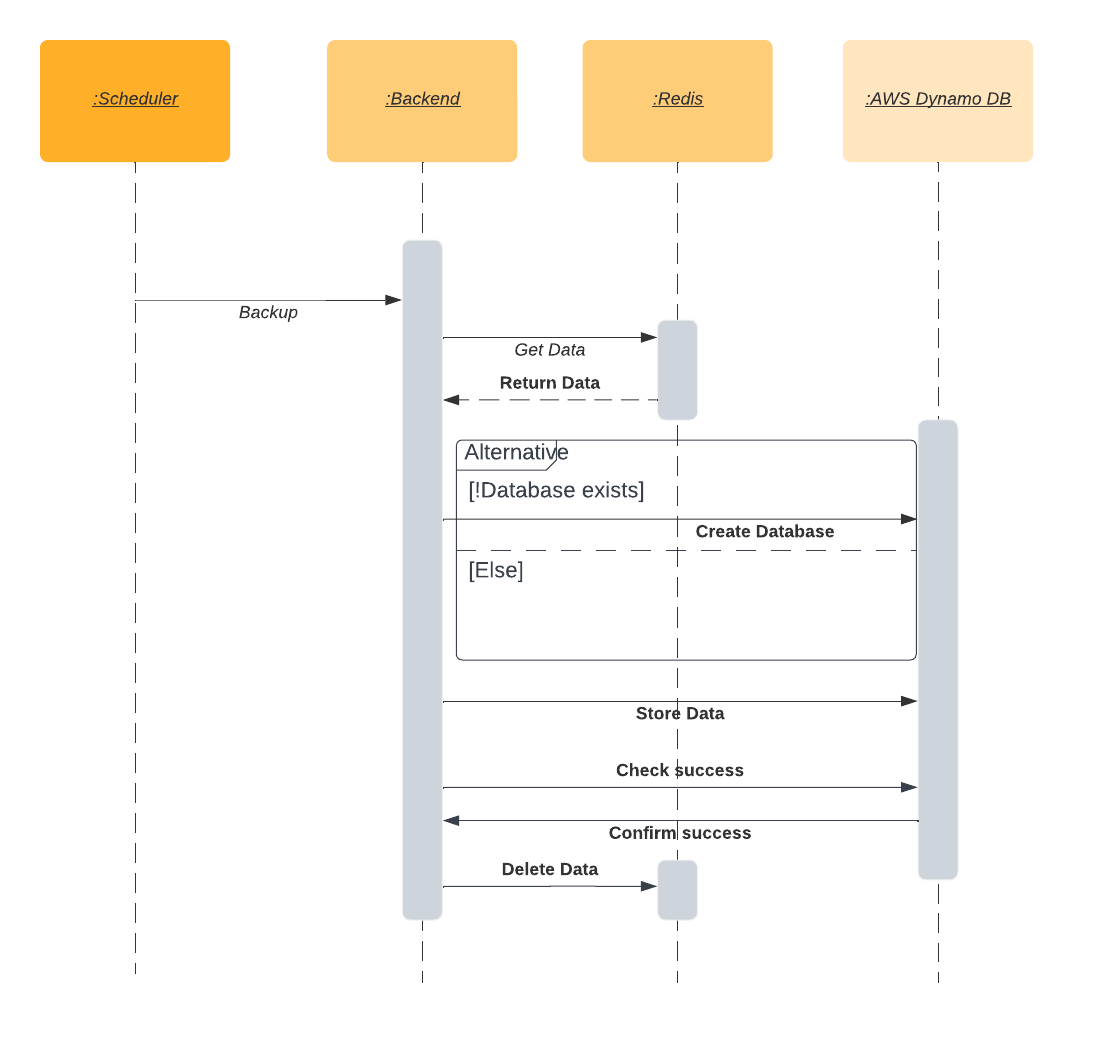
\includegraphics[width=0.8\textwidth]{images/archival_backup.png} 
    \caption{\footnotesize{Archival Cronjob}}
    \label{fig:archival_backup}
\end{figure}

Finally the archival process came as a cronjob shown in figure \ref{fig:archival_backup},
that would take the data each day at 00:00 and archive it from the redis database to the
DynamoDB while checking that everything was successfully archived before cleaning the data
from Redis.



\subsection {File storage Database}
For this second database, that is more opted to be used for the storage of files.
The solution was already known, and was the Amazon S3 service.

The file storage database was used for the following:

    \begin{itemize}
        \item Storing site configuration files
        \item Storing client files
    \end{itemize}

The storage was pretty simple, it was just a bucket with a specific folder structure.
So for the first case it was a folder for each site,
and for the second it was a folder for each client which was handled with the archival
cronjob as these files were related to the data from the trucks that have been handled
during the day.

For the tests we used the following:

    \begin{itemize}
        \item Creating a bucket
        \item Creating a folder structure
        \item Adding data to the bucket and finding it
        \item Deleting data from the bucket
        \item Deleting the bucket
    \end{itemize}

For the creation of the bucket it was made such as it's done automatically once the
server started in case it doesn't exist.
So that we can reproduce the same bucket that there was in the dev environment and during
the  tests.


\section {Security and Authentication}

\subsection {Ratelimiting} \label{subsec:ratelimiting}
rate limiting was one interesting aspect for security, as it's a way to prevent the
server from being flooded with requests. As it could stop DDOS attacks, brute force
attacks, and any other kind of attack that would require sending lot of request from 
the same IP or same user.

For the rate limiting, as we were using already a Spring backend we had a couple options
to choose from the first one was Bucket4j, which is a rate limiter that relies on token
bucket algorithm which approaches rate limiting through putting a number of tokens in a
bucket then whenever the consume or client tries to use a service it has to consume one
or more tokens from the bucket until they are depleted then the client is blocked,
the bucket is then assigned to a key which could be a user, IP address or API key ...

The second option was to use Resilience4j, which relies on creating cycles where each cycle
has a number of allowed permissions and refreshes in the beginning of each cycle, which
allows the handling of the rate limiting in a epoch fashio but it was not easy to
implement for the case of a distributed backend and not worth the trouble to adapt it
with a caching system within the Redis Database to do so, as it relied heavily on
single machines threads for the handling it does.

So we went with the former, which was implemented as a filter within the API gateway
in the Spring backend as shown figure \ref{fig:b4j}.

\begin{figure}[!htpb]
    \centering
    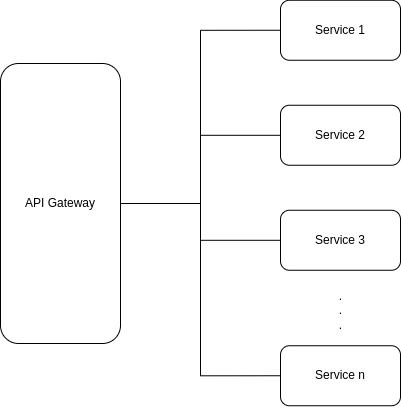
\includegraphics[width=0.5\textwidth]{images/ratelimiting.png}
    \caption{\footnotesize{Backend Gateway}}
    \label{fig:b4j}
\end{figure}


So the now the handling of services within the Java Spring backend required the passage
from API rate limiter which consisted of giving a token to the client before allowing
the request to be processed, and this requests were by default capped to a certain number
that could be modified through the configuration file of the server.

Now with the basic handling in hand, we opt for the implementation of the rate limiter
which was done in two ways, the first was to have a bucket for each user,
and the second was to have a bucket for each IP address.

Rate limiting the user was specifically setup for handling the private endpoints and that
was able to be modified by the admin to allow for more or less requests per second
depending on the user, and the rate limiting the IP address was setup for the public API.

And lastly there was the rate limiting for the login, which was individually handled for
the purpose of limiting the number of login attempts per minute to avoid possibility
of a dictionnary attacks.



\subsection {Authentication}
The authentication was also one of the interesting aspects for security, as it's a way to
prevent confidential data from being accessed without having the right credentials. But the 
prior used solution was having a permanent JWT token that is acquired during the login, meaning 
that once the that Token is generated it could be permanently used to access the data as it didn't
use any additional timing parameter to expire the token.

As for that, came the need to implement a ephemeral token, which is a token that gets expired after
a certain time, to access the data and opted to add a refreshing mechanism which was to make the
user experience better to avoid the need of having them reconnect within their sessions.

But not only that, we also opted to move from a Bearer token transportation of the token to a HTTP Only cookie,
which is a cookie that is only accessible through the HTTP protocol, not the Javascript and is proclaimed to
be the safest option to store the JWT. And then proceeded to embed the token within the cookie,
as so we can avoid the possiblity of exploitation through JS injections to acquire the token.

The authentication had a simple flow \ref{fig:token}, the user presented his credentials,
the server validated them, in case they were valid the server would generate a new access 
token, which was embedded in the header as a HTTP Only cookie then that would make 
all the request coming from the front end to the server to have the token in the header
with no need for the Javascript to do any handling for that last.

\begin{figure}[!htbp]
    \centering
    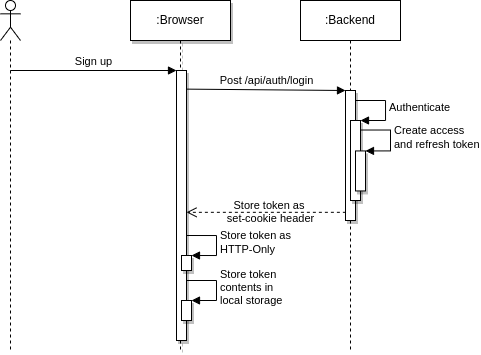
\includegraphics[width=0.75\textwidth]{images/JWTHttpOnly.png}
    \caption{\footnotesize{JWT HTTP Only Cookie}}
    \label{fig:token}
\end{figure}

The refresh token mechanism was to make the user experience better and also to increase
the security of the application, make the intercepted JWT tokens mostly come in useless
if they were caught late, as they would be expired.

So the flow \ref{fig:refresh} of that was to that during the login there was a generation
of access token and refresh token, the referesh token came in handy to create a new access
token once the old one has expired and the user was still active during that session, to
avoid forcing the user to re-login.

\begin{figure}[!htbp]
    \centering
    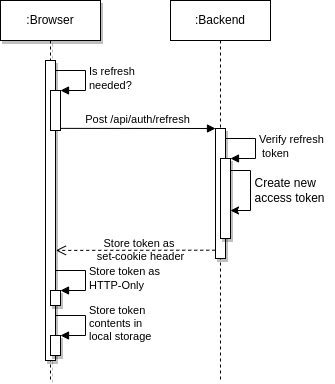
\includegraphics[width=0.42\textwidth]{images/refresh.png}
    \caption{\footnotesize{Refresh token}}
    \label{fig:refresh}
\end{figure}

\newpage


\section {Containerization and Deployment}
Before we dive in into the specifics, we first will showcase the final architecture in the
Elastic Container Service (ECS), which is a fully managed container orchestration service,
more information about the ECS can be found in the following link \cite{ecs_intro}

\begin{figure}[!ht]
    \centering
    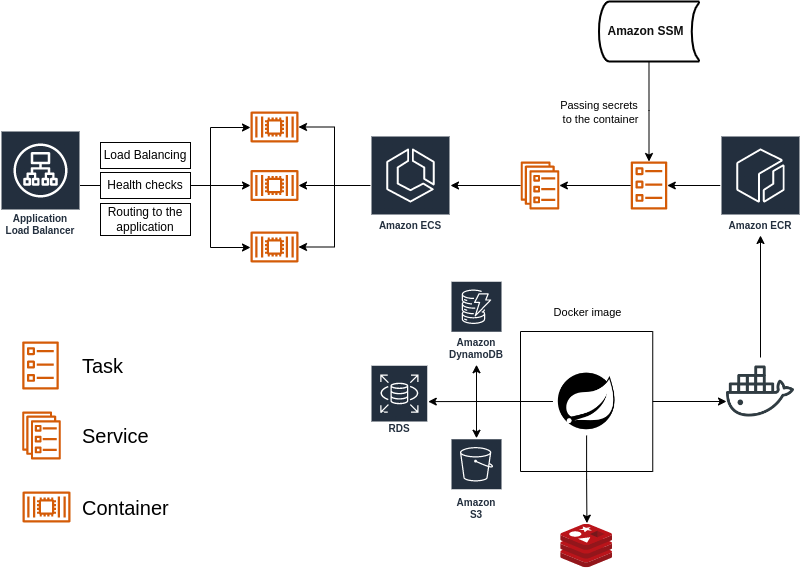
\includegraphics[width=\textwidth]{images/ECS}
    \caption{\footnotesize{ECS Architecture}}
    \label{fig:ECSArch}
\end{figure}

Task: the component which takes care of running the containers.

Service: the component which manages the tasks.

Container: the image that is running on the task.

\subsection {ECS Containerization and secrets}

The ECS solution shown in figure \ref{fig:ECSArch} was a bit of a challenge to get it to
work, as it was a containerized solution, and not a native one.
So the first step was to containerize the solution, and have a safe image that doesn't
expose any secrets or environment variables.

In the docker way, we can just pass them through the command line,
and the solution will run perfectly.

But here relied a problem that was the ECS solution, it didn't have a simple
way to feed it the credentials, environment variables neither files, so we had to opt
for using the SSM or Secrets Manager
which is yet another hosted solution to store strings as secrets, and then those could be 
passed to the ECS services.

With the Secrets Manager, for the strings secrets it was a simple writing / reading process
to store and retrieve the secrets. But for the files it was a bit more complicated, there
wasn't a direct way to do that.

Finally we came up with the following solution, which is as follows:

\begin{itemize}
    \item Serialize the content of the file into a base64 string
    \item Store the base64 string in the AWS Systems Manager (SSM)
    \item Pass the SSM secret to the ECS service
    \item Retrieve the secret from the SSM as a environment variable
    \item Decode the base64 string
    \item Store the deserialized base64 in a file in the container
    \item Point an environment variable to the file
\end{itemize}

As such we managed to pass aws credentials, google credentials and Redis Labs credentials.

\subsection {Load Balancer and routing}

As shown in the ECS Architecture, we had a load balancer in front of the running tasks, which has four main goals:

\begin{itemize}
    \item To take care of the incoming traffic from the client side
    \item To ensure that the traffic distributed evenly
    \item To ensure that the tasks are healthy
    \item To ensure that the tasks are not overloaded and manage it's scalability.
\end{itemize}

\begin{figure}[!htbp]
    \centering
    \includegraphics[width=\textwidth]{images/loadBalancer.png}
    \caption{\footnotesize{Load Balancer Interaction with the backend}}
    \label{fig:loadbalancer}
\end{figure}

So the load balancer is as shown in figure \ref{fig:loadbalancer}, it took traffic from
port 80 where it had an exposed dns link, then it routed it through a VPS to the
containers that are exposing post 8080 in their local network, having healthchecks
done on the endpoint /actuator/health .

With that set in place, we had pretty much everything setup to start testing for the
load handling by the ecs to check for the health of the containers and the measures
to be set to ensure that the auto scaling is setup with the right parameters.

So first, we written scripts that did kind of overload the server with the requests,
asynchronously deploy the containers and check monitoring metrics.

\begin{figure}[!ht]
    \centering
    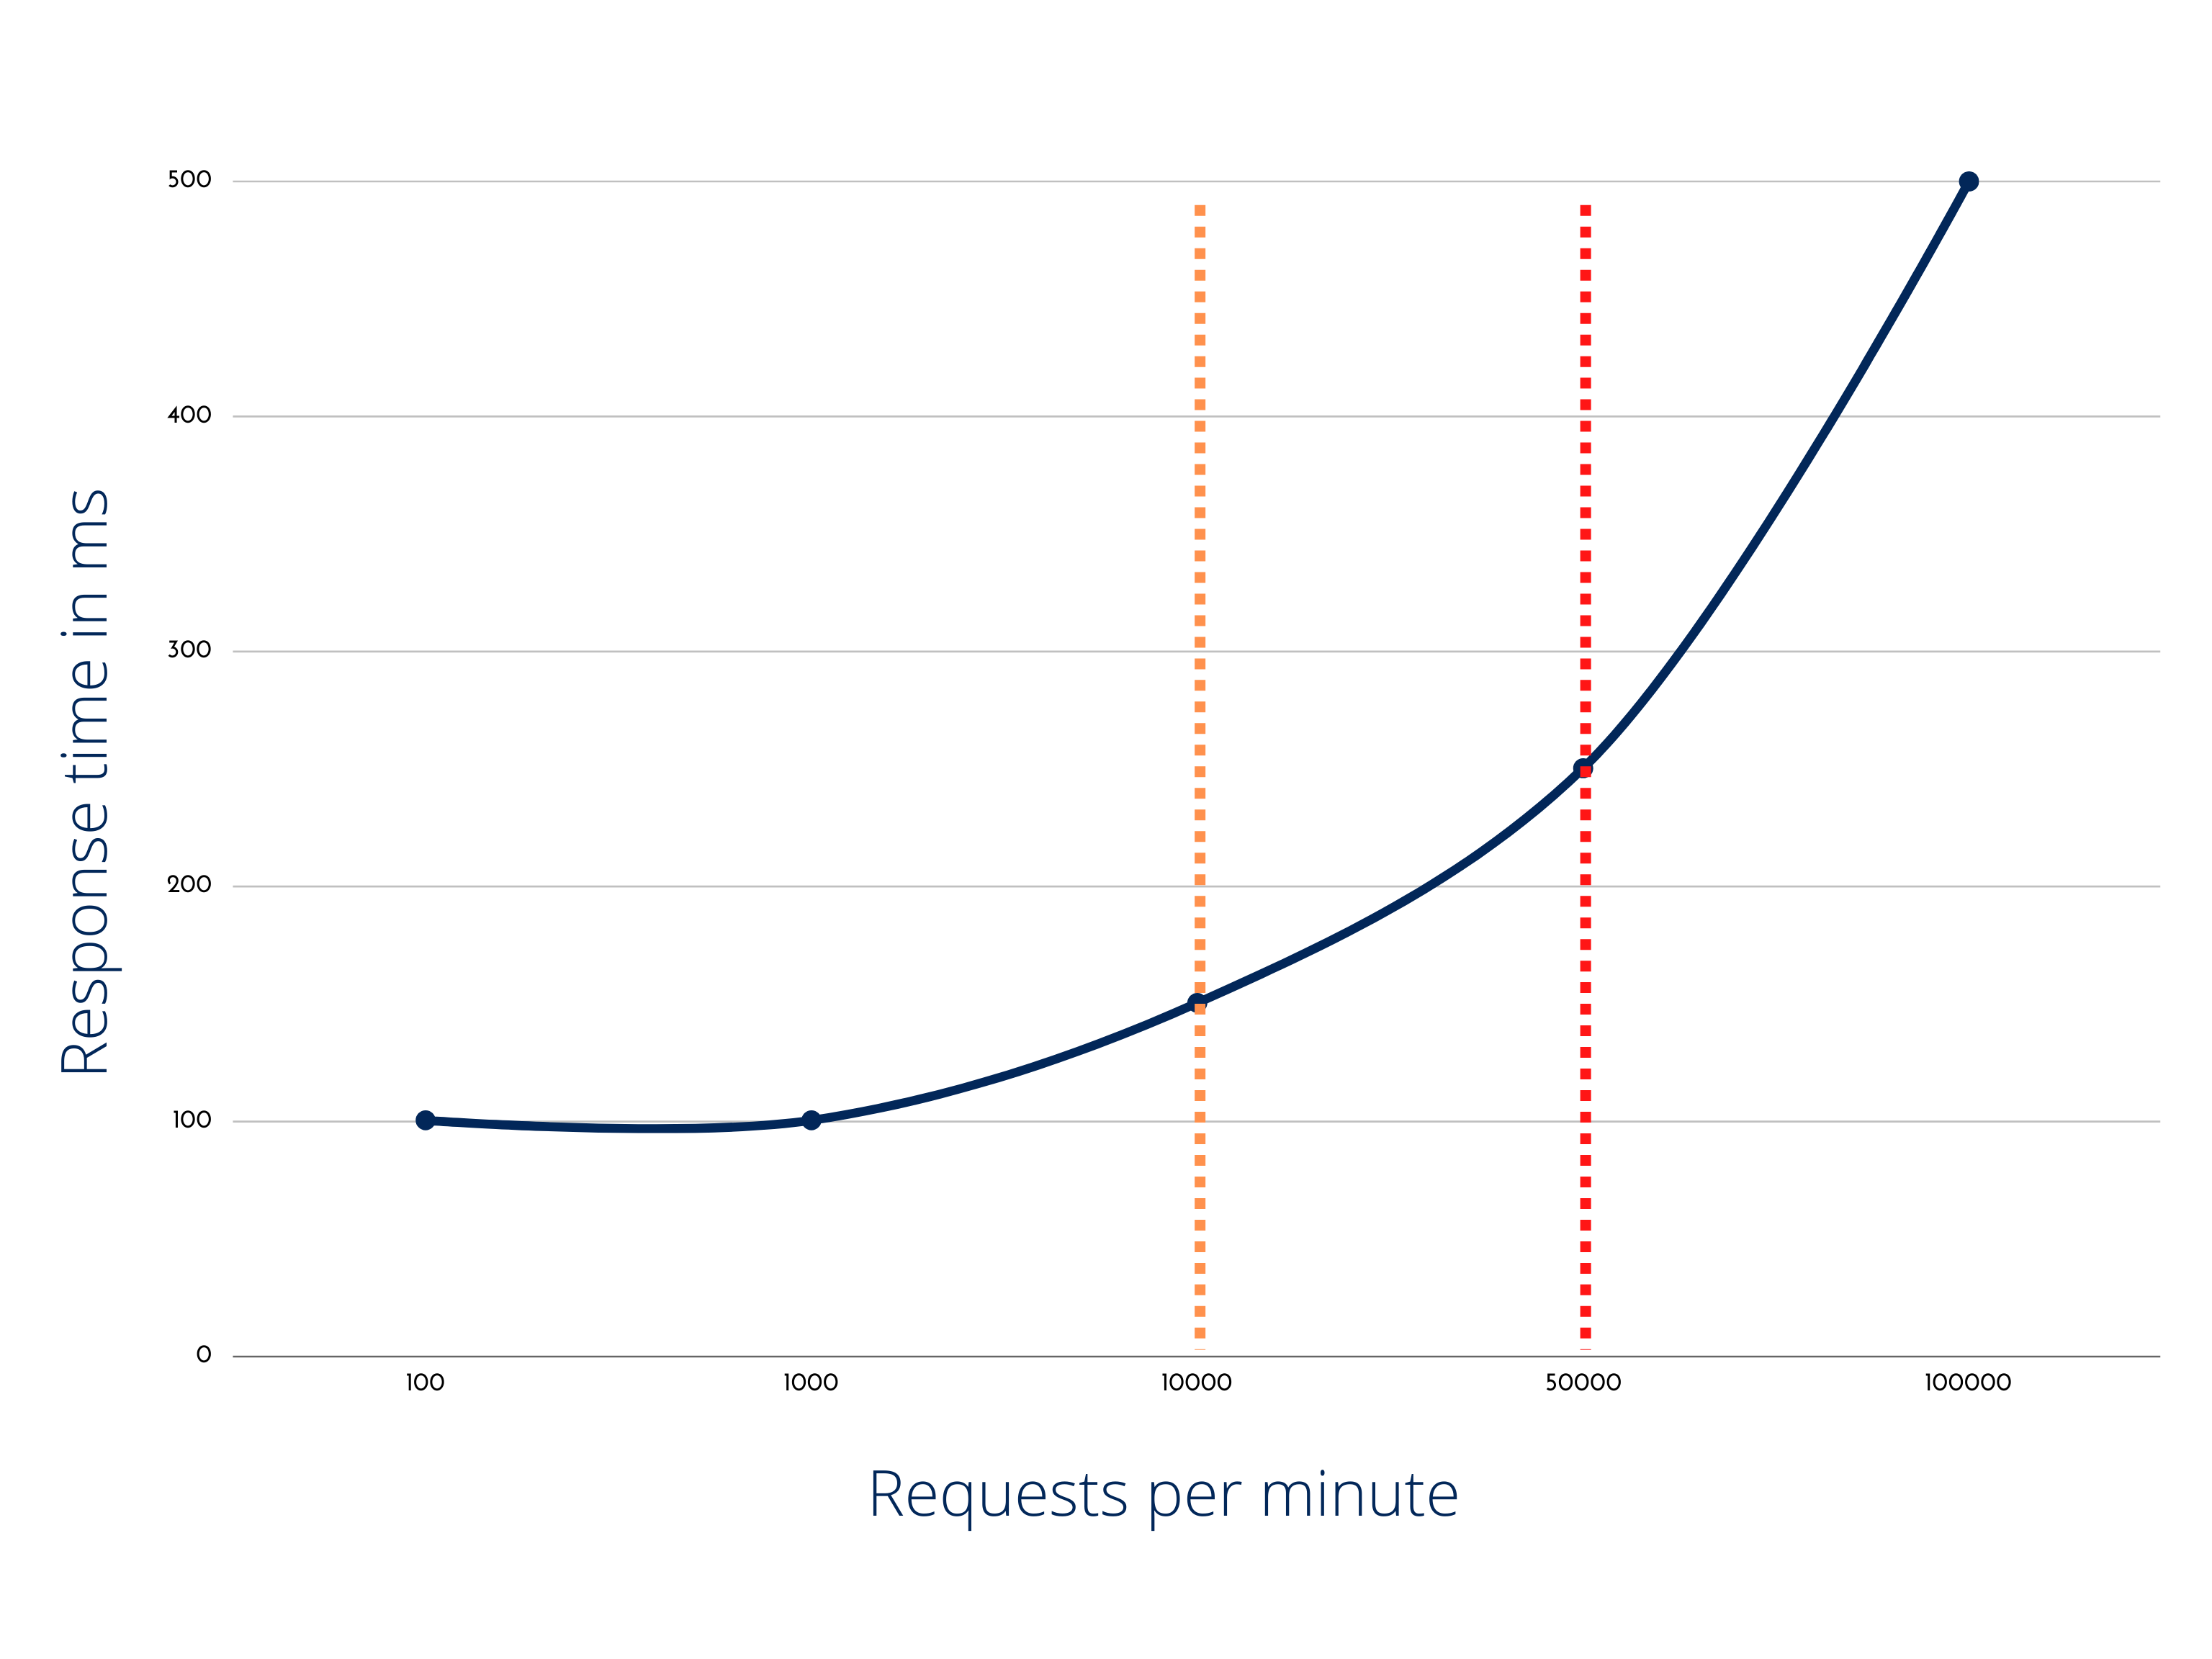
\includegraphics[width=\textwidth]{images/assesment_autoscaling.png}
    \caption{\footnotesize{Auto Scaling Assessment}}
    \label{fig:autoscaling_assessment}
\end{figure}

So next came doing the assessment of autoscaling, we ended up compiling the chart
in figure \ref{fig:autoscaling_assessment} which shows the response time per
number of requests sent per minute, the assesment was done by using a script
written in Scala.
Looking at the chart we can see that the response time was pretty stable until
we reached the 10000 requests mark, where there was a clear increase but nothing
that could kill the usage till we exceeded the 50000 mark where the response time
was getting really high meaning that at this point there's no advantage on keeping
only the existing instances up but the need to increase becomes apparent, and that
was due to the heavy requests creating a sort of queue in the backend which would
require multiple processes thus comes the horizontal increase advantage in the ECS.

So firstly, as shown in \ref{fig:loadtest} it took the endpoint to be hit, in case
it was a private endpoint you'd need to provide the credentials to. Then put in place
the number of requests to be sent and finally run it.

Once it started running it was a simple case of sending requests asynchronously in fibers
or virtual threads, and then printing the response time of each request, as such we could
monitor the handling time of the requests being affected by the load of requests.

\begin{figure}[!ht]
    \centering
    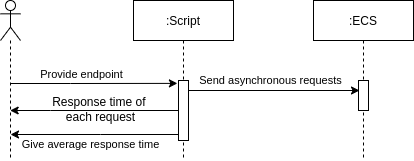
\includegraphics[width=0.8\textwidth]{images/scriptdos.png}
    \caption{\footnotesize{Load Test Script}}
    \label{fig:loadtest}
\end{figure}


Thus it we could find the right parameters for the autoscaling, based on the number of
requests being sent per minute, which at the time of tests was around 50000 requests per
minute without the response time being affected which is quite impressive.

And as most the back-end services relying heavily on the memory, we ensured to put a 70\%
memory usage limit on the containers before spawning new instances to handle the load, in
case of autoscaling by memory.

Next came the assesment and benchmarking of two databases solutions which were a Redis
instance hosted in EC2, and a Redislabs hosted instance.

The tests were done by using a script that was written in python, and it was a
stress testing script, which sole purpose was to overload the Redis instance 
and then check if the requests then took longer to fulfill, as Redis was a in-memory
database, so the goal of using it was speed.

\begin{table}[!ht]
    \centering
    \begin{tabular}{| c | c |}
        \hline
        \textbf{Database} & \textbf{Stress Test} \\
        \hline
        Redis on EC2 & 
                \begin{tabular}{| c | c |}
                    \textbf{Load} & \textbf{Response by Endpoint} \\
                    \hline
                    \textbf{25\%} &
                            \begin{tabular}{| c | c |}
                                \textbf{Endpoint} & \textbf{Response Time} \\
                                \hline
                                Add client & \textbf{129.9} \\
                                \hline
                                Get all clients & \textbf{89.9} \\
                                \hline
                                Heavy Load Enpoint & \textbf{269.2} \\
                            \end{tabular}\\
                    \hline
                    \textbf{50\%} &
                            \begin{tabular}{| c | c |}
                                \textbf{Endpoint} & \textbf{Response Time} \\
                                \hline
                                Add client & \textbf{128.3} \\
                                \hline
                                Get all clients & \textbf{106.1} \\
                                \hline
                                Heavy Load Enpoint & \textbf{245.7} \\
                            \end{tabular}\\
                    \hline
                    \textbf{75\%} &
                            \begin{tabular}{| c | c |}
                                \textbf{Endpoint} & \textbf{Response Time} \\
                                \hline
                                Add client & \textbf{133.6} \\
                                \hline
                                Get all clients & \textbf{196.1} \\
                                \hline
                                Heavy Load Enpoint & \textbf{257.7} \\
                                \hline
                            \end{tabular}\\
                \end{tabular}\\
        \hline
        Redis on RedisLab & 
                \begin{tabular}{| c | c |}
                    \textbf{Load} & \textbf{Response by Endpoint} \\
                    \hline
                    \textbf{25\%} &
                            \begin{tabular}{| c | c |}
                                \textbf{Endpoint} & \textbf{Response Time} \\
                                \hline
                                Add client & \textbf{154.1} \\
                                \hline
                                Get all clients & \textbf{79.5} \\
                                \hline
                                Heavy Load Enpoint & \textbf{256.8} \\
                            \end{tabular}\\
                    \hline
                    \textbf{50\%} &
                            \begin{tabular}{| c | c |}
                                \textbf{Endpoint} & \textbf{Response Time} \\
                                \hline
                                Add client & \textbf{134.1} \\
                                \hline
                                Get all clients & \textbf{126.4} \\
                                \hline
                                Heavy Load Enpoint & \textbf{241.2} \\
                            \end{tabular}\\
                    \hline
                    \textbf{75\%} &
                            \begin{tabular}{| c | c |}
                                \textbf{Endpoint} & \textbf{Response Time} \\
                                \hline
                                Add client & \textbf{143.5} \\
                                \hline
                                Get all clients & \textbf{156.3} \\
                                \hline
                                Heavy Load Enpoint & \textbf{258.2} \\
                                \hline
                            \end{tabular}\\
                \end{tabular}\\
        \hline
    \end{tabular}
    \caption{\footnotesize{Stress testing Redis against RedisLab}}
    \label{tab:stress_testing}
\end{table}

The results on the table above were quite impressive, as the response time of the
requests was quite low, and the load was quite high, the only noticeable growth was
in the response time of the Get All Clients and that was due to the fact that to 
increase the load on the Redis instance we had to increase the number of clients.
Thus, get all clients got heavier and heavier to handle.

As shown in \ref{tab:stress_testing}, it ended up being with a pretty close result,
no one over ruling the other, and the results were pretty close to the expected results.
So we ended up either having to opt for the Redis instance hosted in EC2 and do 
all the configuration manually which would lead to a lot of configuration done manually,
or just resorting to the Redislabs hosted instance, as it's a fully managed instance.
All the security measures and replication are taken care of by cloud host.

\subsection{Deployment}

Finally after testing everything, and having deployed one ECS service succesfully, we had
to automate the deployment process, so that we could handle new versions and code update
without much effort.

This came in the form of a gradle task, which was as follows:

    \begin{figure}[!htbp]
        \centering
        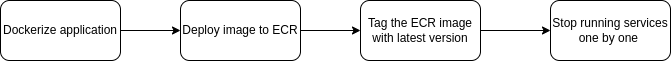
\includegraphics[width=\textwidth]{images/gradle.png}
        \caption{\footnotesize{Deployment of the App to ECS - Gradle Task}}
        \label{fig:gradle}
    \end{figure}

The dockerization part of the gradle task was handled using a third party plugin,
then the deployment to Elastic Container Registry (ECR\footnote{ECR is an AWS managed
    container image registry service that is secure, scalable, and reliable. More
    information can be found in \cite{ecr_intro}.})e using the AWS CLI,
by linking the ECR to docker, then pushing the image is automatically uploaded to ECR.
Once this is done, the ECS service has to handle the update of the image, 
and this was done through a bash script that took in charge of getting a list 
of the running tasks, then stopping one of them, and wait for a new one to spawn 
such as to avoid down time during the update of the service.

    \begin{figure}[!ht]
        \centering
        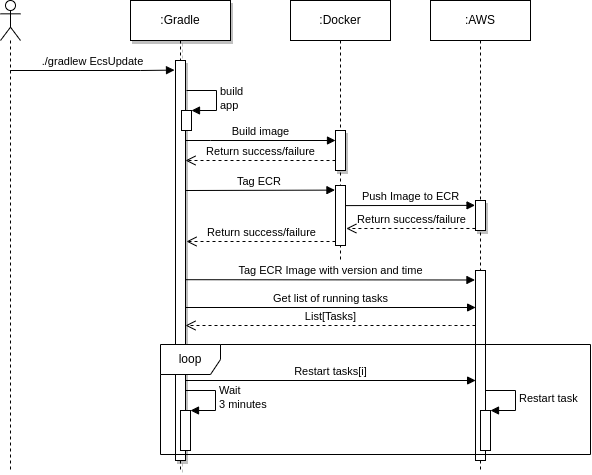
\includegraphics[width=0.9\textwidth]{images/gradleTask.png}
        \caption{\footnotesize{Deployment Sequence Diagram}}
        \label{fig:deployment}
    \end{figure}

So in the figure \ref{fig:deployment}, the flow is pretty simple,
it goes as follows:

    \begin{itemize}
        \item Gradle builds the docker image using a 3rd party plugin
        \item Tag image with right version of the application and push it to ECR
        \item Tag ECR image with current version in addition to timestamp it
        \item Get the list of running tasks
        \item Stop one of the running tasks
        \item Wait for a new one to spawn
        \item The two last steps are repeated till the list is exhausted
    \end{itemize}

And in such a way, we can handle the deployment without having any downtime,
so it makes introducing bug fixes a better experience for both developer and 
customer.



\section {Continuous Integration}
\subsection{What is continuous integration?}

Continuous integration(CI) is a technique for building software incrementally, as in a way
to automate the build and testing of the code. This method encourages developers to 
write code that is more readable, more maintainable, and more testable. Also it makes
it easier to find bugs before they are introducted into the main code, and to
catch as much problems as possible before the code reaches the production environment.

CI has emerged as a great tool for software development, as it eases the process of
merging code from different branches which allows for a more efficient development process,
as developers mostly work on their own branch in isolation, and this allows them to 
introduce features and fixes that integrate with the rest of the code. \cite{ci_msft}

Along with CI, there is Continuous Delivery(CD), which is the other end of this process
and is used to push code to a production environment, allowing for smoother introduction
of updates, hotfixes, \dots

\subsection{CI/CD projected on the system}

As one of the most important features within the industrialization of the project
was having a reliable and maintainable deployment process, here where came the 
continuous intagration pipelines. The CI pipeline offered a great way to have
a reliable and maintainable deployment process and to automate the whole process
of the project.

\begin{figure}[!htpb]
    \centering
    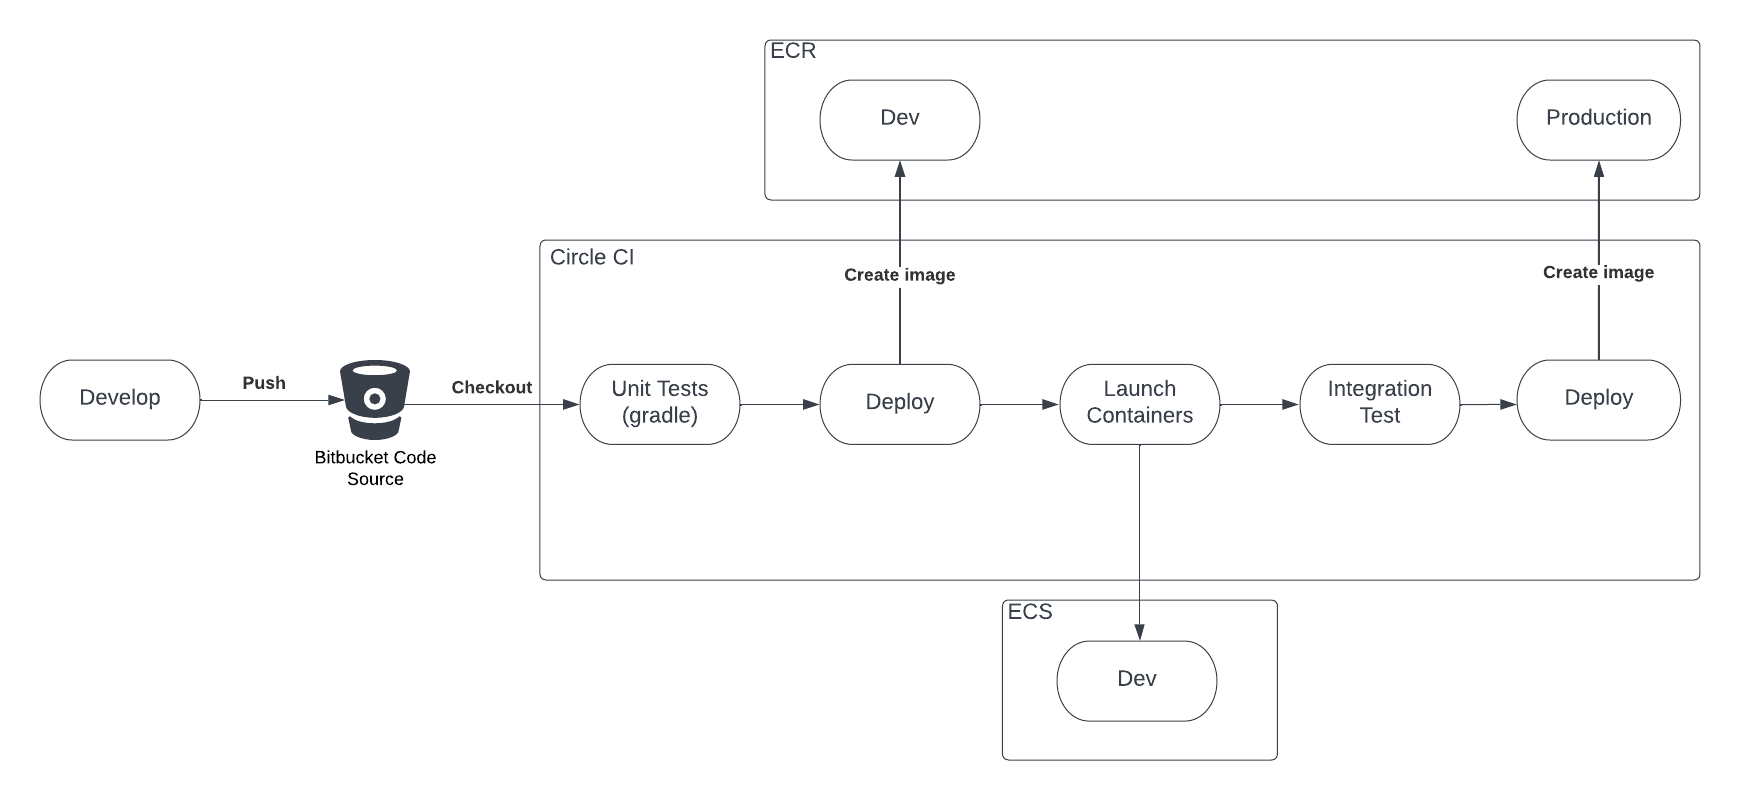
\includegraphics[width=\textwidth]{images/ci-cd-pipeline.png}
    \caption{Continuous integration pipeline}
    \label{fig:ci-cd-pipeline}
\end{figure}

As shown in the figure \ref{fig:ci-cd-pipeline}, the CI pipeline is composed
of three main steps:
    \begin{itemize}
        \item \textbf{Test}: the test phase is the first step of the CI pipeline.
            It is responsible for running the tests built on the project using
            the gradle test task.
        \item \textbf{Coverage}: the coverage phase is the second step of the CI pipeline.
            It uses SonarScanner, which is a scanner for code analytics reporting things
            from code quality to security threats. It generates the coverage report of the
            project and then it sends the report to the SonarCloud\footnote{SonarCloud is
                a cloud service used for hosting SonarQube scans} server.
        \item \textbf{Build and Deploy}: the build and deploy phase is the last step
            of the CI pipeline. It is responsible for building a docker image and then
            pushing it to ECR (EC Container Registry) and then deployed to ECS
            (ECS Container Service) all that using a range of custom scripts built
            by us within gradle, to ease up the deployment within the pipeline.
    \end{itemize}

The CI/CD service we've went for was the Circle CI, which is a hosted continuous
integration service that is used to test the code and to deploy the application.
The configuration of the CI/CD service was configured within a yaml file,
which is located in the \texttt{.circleci/config.yml} file.

The test and building steps both came from taking advantage of the gradle build
system, which were already setup and configured within the project. But nonetheless,
as the CI/CD pipeline creates docker containers to run the tests and the build,
and the tests needed AWS credentials to be able to run, we had to somehow pass
the file containing the AWS credentials to the CI/CD pipeline, which was done
by creating new AWS credentials creating a AWS credentials file then encoding to
base64 and passing it to the CI/CD pipeline as a environment variable, then decoding
it to a string to be stored in the \texttt{.aws/credentials} inside the pipeline which
was a play around to pass the files to any virtualized environment not allowing for 
those accesses.

Next came the coverage phase, which was a bit more involved. The coverage takes care
of analyzing the code to see if there are any security issues, bugs, bad code and
everything that relate to code analysis, and then it sends the report to the
SonarCloud server. The important thing in this phase is that it can be as a test to
the code's quality, so you can set the threshold of the coverage to be a certain
percentage, and if the coverage is below that threshold, then the CI/CD pipeline
will fail so we can stop critical issues from being deployed if they weren't caught
during development.

The deployment, which is the last step of the CI pipeline, is done using orbs
within Circle CI, orbs are snippets of codes used to automate repeatable processes
and published by the Circle CI team, specifically the ECR and ECS orbs.

As the orbs didn't come in handy, as we had different way of building the docker image
than the default one, we opted to creating our own job within the CI/CD pipeline
which took care of the building and deployment phase of the project.
The job went as follow: 
    \begin{itemize}
        \item Create a docker image using the gradle build tool.
        \item Tag the docker image with the project name.
        \item Push the docker image to ECR.
        \item Set ECR image with the right tags.
        \item Restart the ECS running tasks to run the new image.
    \end{itemize}

In the end, the CI/CD pipeline was configured to only build and deploy on two branches
which are "master" to deploy on the production environment and "dev" to deploy on the
development environment.


\section {Refactoring and Improvements}\label{sec:refactoring}
\subsection {Adding user management system}

The old system didn't have a user management system, as it relied on the site being the
user so there wasn't really users to manage. So we had to integrate users within the system
then add a way to manage them, and this was done by migrating the site from being the user
to being an entity that could be managed by users who have the right to do so.
And that required rework through the majority of the backend as this architecture was
relied on by all the backend services and controller and also frontend.

So we had to change this architecture to be able to manage users and their roles, but also
keep the old behaviour the same.

%TODO: Add class diagram before and after (Couldn't do it now because we migrated directly without using diagrams)

\subsection {Implementation of tests for existing codebase}

TODO: Still not touched on yet


\section {Conclusion}

To conclude, during the implementation of the subjects, we had implemented a lot of
new features and improvements ranging from databases and security, to infrastructure 
and deployment.
As we've seen during the last section \ref{sec:refactoring}, the refactoring wasn't 
implemented yet, but the main goal of this phase has been discussed in such a way
that it will be easier to implement the refactoring in the future.
The main goal of this contributions phase was to make the ground work for a more rigid
and upgradable solution, which would allow for the development of a more robust and
upgradable solution once the refactoring is fully implemented.



    \chapter{Simulation}\label{sec:simulation}
    In this chapter we'll have a brief showcase of the project, and where the modules
I've been working on are located within.

Firstly we'll have a brief look at the East Truck In (ETI) interface, which is 
the main interface for the project. We'll specifically look into the user management
aspect.

\begin{figure}[!ht]
    \centering
    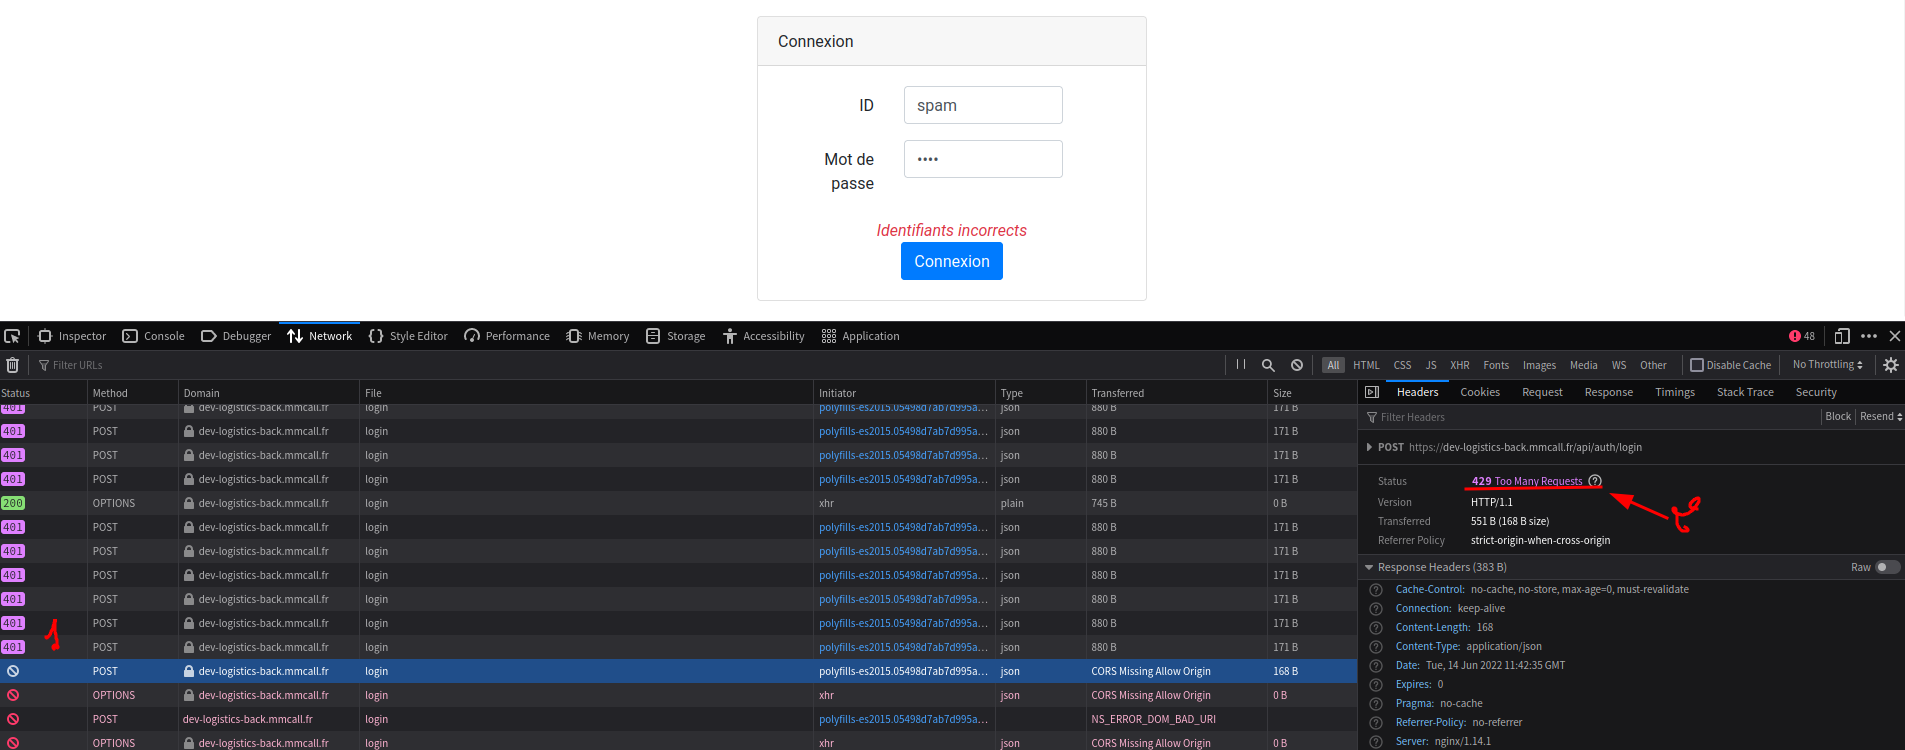
\includegraphics[width=\textwidth]{images/login too much attempts}
    \caption{Login requests stopped after too much attempts}
    \label{fig:login_req_ratelimit}
\end{figure}

In the figure \ref{fig:login_req_ratelimit} we can see that the login requests after a
certain number of attempts where the login was erroneous in purpose started getting
error 429, which is due to  the API rate limiter being triggered as we've discussed in
section \ref{subsec:ratelimiting}.

Next we'll take a look at the \ref{subsec:user_management} section, which is the
update of the user's profile, to make it easier to manage roles and have a overall easier
to use system.

\begin{figure}[!ht]
    \centering
    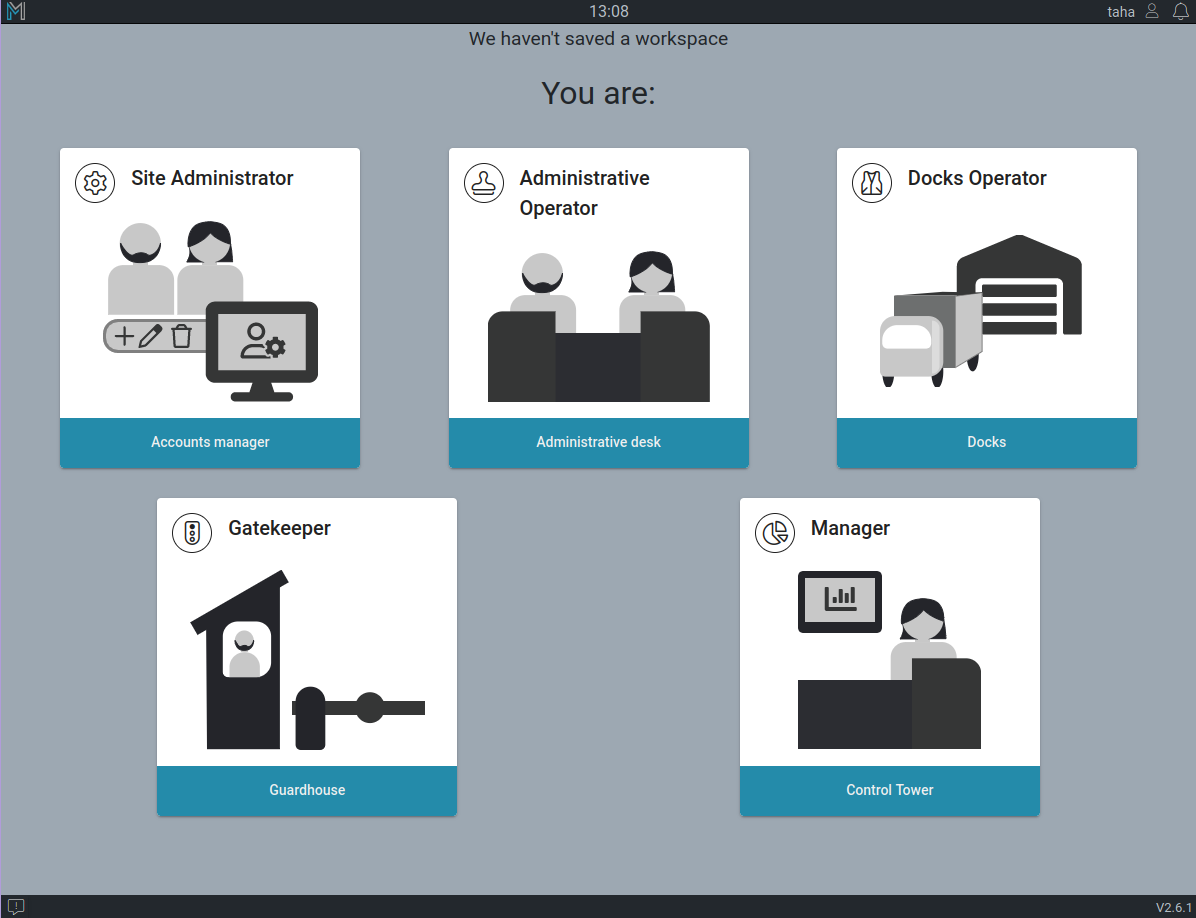
\includegraphics[width=0.49\textwidth]{images/user management}\hfill
    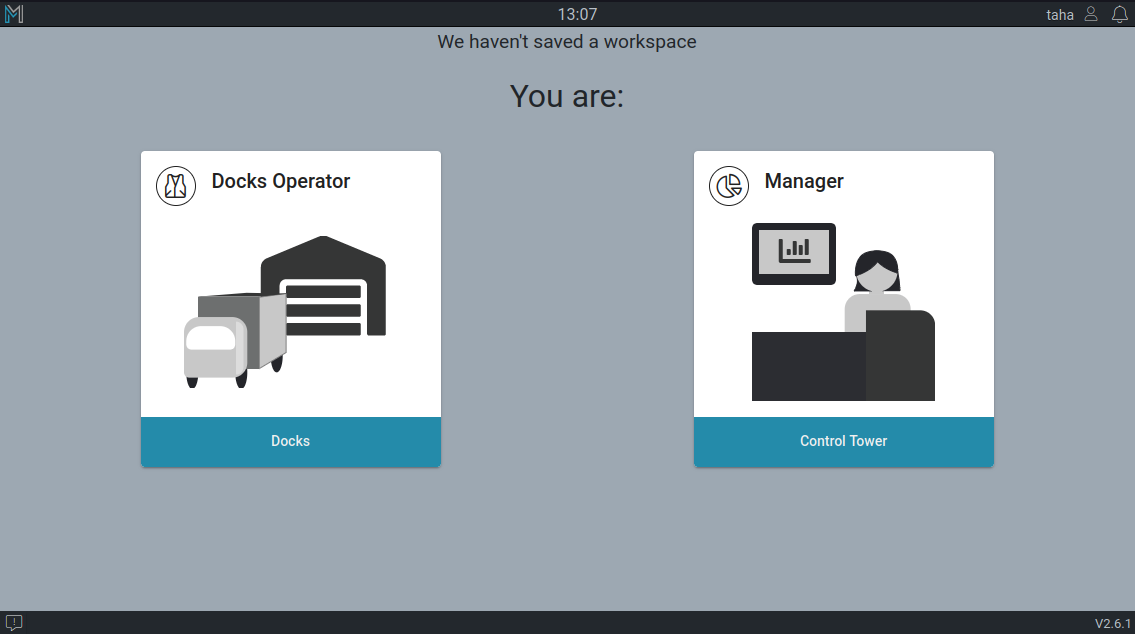
\includegraphics[width=0.49\textwidth]{images/userLessRoles}
    \caption{ETI Main Page}
    \label{fig:user_management_view}
\end{figure}

So the main view of the user management interface is the one in the figure
\ref{fig:user_management_view} which is a list of all workspaces available to the current
user, in my case I have access to all five workspaces.

So by removing a couple of workspaces from the current user from the database,
we can see that the user management interface is also updated and the workspaces
access change and that's due to the user management module we've implemented.

So here in 2nd figure \ref{fig:user_management_view}, we removed three workspaces from
the current user and we have access to only two workspaces.

So this access control is only doable by two types of users, the ones with the roles
of \textit{admin} which is a superuser and users who have the access role of
\textit{Account Manager} which is a user who can manage the accounts of other users.
From creating a new user to deleting a user, and they are related to the site.

\begin{figure}[!ht]
    \centering
    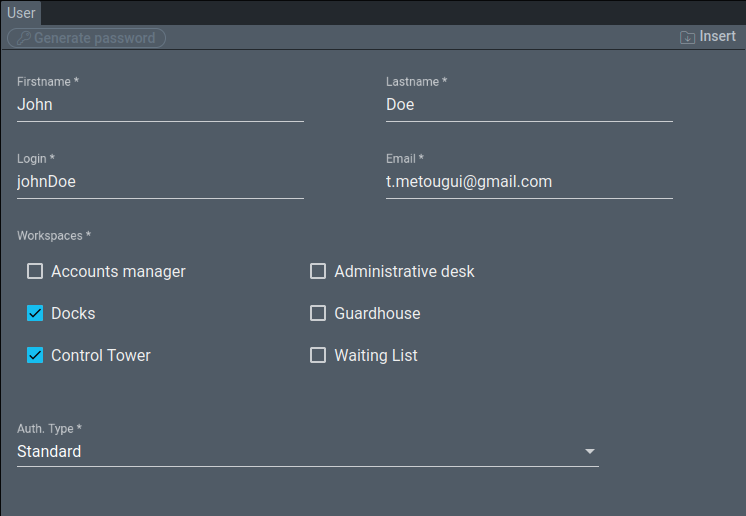
\includegraphics[width=0.49\textwidth]{images/insertingANewUser}
    \hfill
    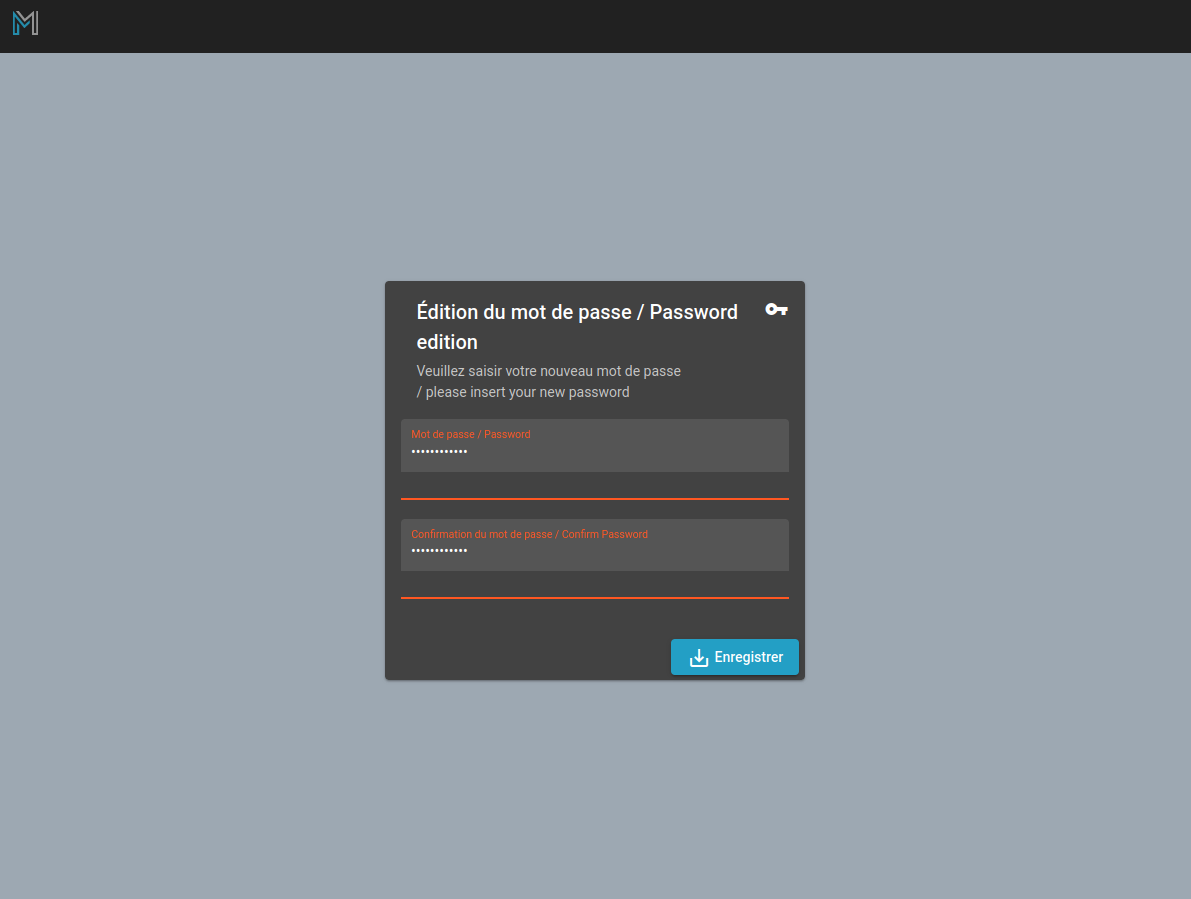
\includegraphics[width=0.49\textwidth]{images/password}
    \caption{Adding a new user}
    \label{fig:insert_user}
\end{figure}

The figure \ref{fig:insert_user} shows the part in account management where we can add
a new user to the system. Giving power to control his roles and workspaces.

\begin{figure}[!ht]
    \centering
    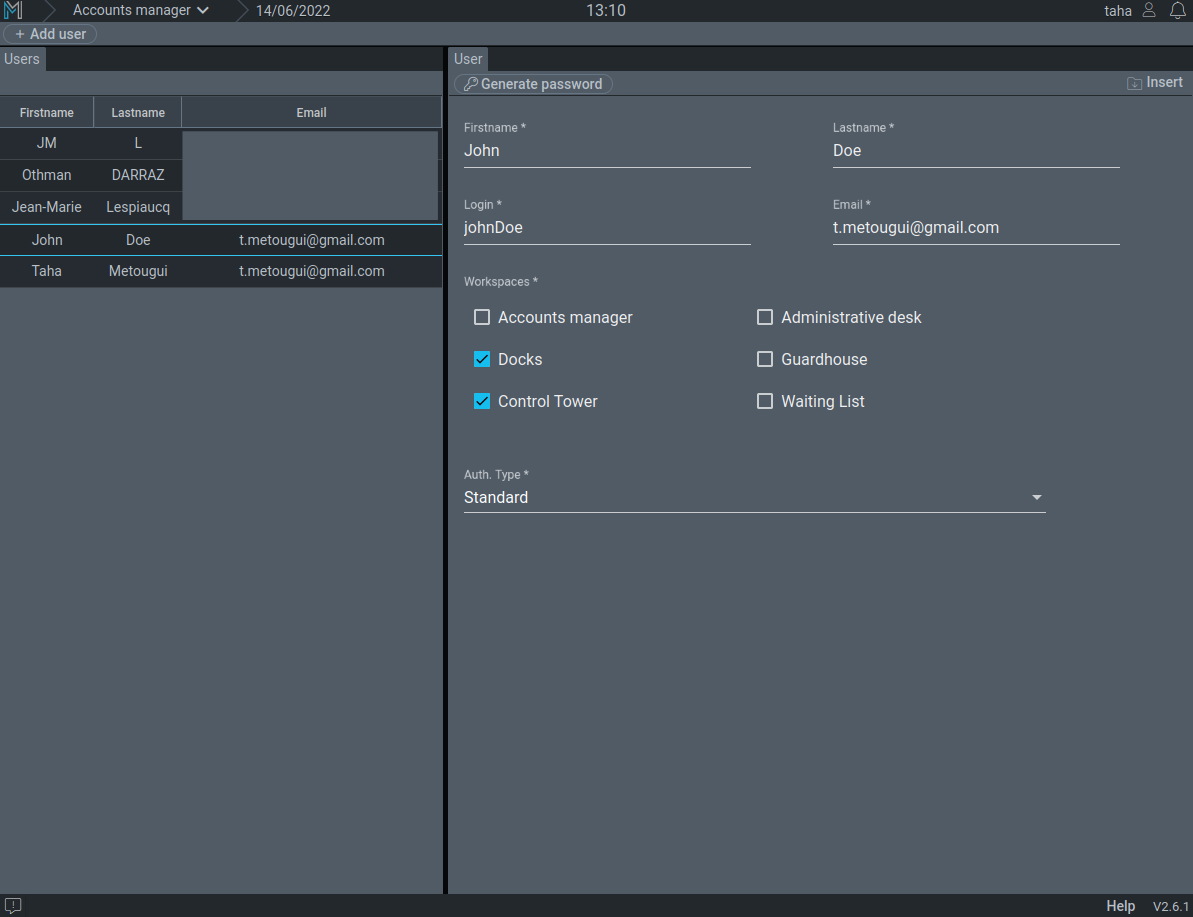
\includegraphics[width=\textwidth]{images/accManager}
    \caption{Account Manager}
    \label{fig:accManager}
\end{figure}

Once added the user is shown in the list of users, on the side of the page. As shown in 
figure \ref{fig:accManager} where we can see all the users that are in the site the 
current user is in.

Once user added, we get the possibility to create a new password for the user. By clicking
the generate password button, then a email is sent to the user and then you receive the
email in your inbox that redirects you to a page in 2nd figure \ref{fig:insert_user} where
it can be seen that the client gets invited to introduce their password.
Such a mechanism is put in place because the users can only be created by account managers.

As for the rest of the workspaces their business logic is mostly for the fleet management, 
and wasn't in the scope of my implementation except for creating roles for those workspaces
to be accessible.



    \chapter{General Conclusion}\label{sec:conclusion}
    To summarize, during the course of the project, I have taken part in adapting an MVP
for logistics, specifically the management of trucks and their drivers within the 
warehouse with the organisation MMSoft, to SaaS standards and turn it to a competitive
product within the market. The initial solution was more a proof of concept with the 
capability for real usage, but missing the security, scalability and maintainability
requirements. So we undertook a full-fledged project with the following goals:
    \begin{itemize}
        \item Implement archival capabilities to store the data in a database.
        \item Implement security features, such as rate limiting and update the authorization system.
        \item Migrate the product to a scalable and rigid infrastructure, with automated scaling.
        \item Adding Continuous Integration and Continuous Delivery to multiple levels.
        \item Refactoring the code to make it more readable and maintainable.
    \end{itemize}

The project was took up by a team of three people, handling the tasks with
the kanban method, which had five states:
    \begin{itemize}
        \item Stand-by
        \item Request
        \item In progress
        \item To Review
        \item Done
    \end{itemize}

The implemetation of the project for multiple of the goals has been a success, for
the most part. So far, the archival has been implemented within the AWS database
DynamoDB, and S3 for the files archival. The security has took turn into moving 
the JWT Bearer token transfer to a cookie based system, where the token is stored
in the browser as a HTTP Only cookie, then within the same subject we had API 
rate limiting, which was implemented using Bucket4J library within the filter layer
of the API gateway. The infrastructure took a transfer from the EC2 instance to 
a ECS cluster, which allows for better scalability and maintenance for the running 
system. The CI/CD has been implemented using the Circle CI hosted service,
with the help of quality gateways offered by Sonarqube to assess the quality of the
code to allow it to pass or not.
The tests have been implemented using the JUnit and Mockito libraries, and the
implementation of the API has been done using the Spring Framework.
For each step or task of the project, we were implementing unit tests or ensuring
functionality of the task with manual tests, before moving it to the "To review" state
within the kanban board.
The reviewing of the project was done by the product owner, who is the CEO and 
knows how exactly the product should be implemented for the clients needs.

Of course, the project was not completed to a 100\% in the time allotted, so the
limits reside currently in the scope of the performance of some endpoints 
that rely on pulling big sets of data from the Redis Database and which is currently
being investigated for a better implementation. The refactoring part of the project
is still heavily in progress, as there are still many decisions to be made regarding
the technologies to use and the way to implement them before diving into it.

So for the future of the project, it would be clear that targetting the refactoring
of the code base would be the best way to improve the project, as it would open 
doors for easier implementation of the new features and have some significant improvement
in the performance of some services.


    \backmatter

    \printbibliography[title=References]
    \addcontentsline{toc}{chapter}{Bibliography}

    \appendix

\end{document}
